\documentclass[10pt,a4paper]{article}

% ── Paquetes ──
\usepackage[utf8]{inputenc}
\usepackage[T1]{fontenc}
\usepackage[spanish]{babel}
\usepackage{geometry}
\usepackage{graphicx}
\usepackage{array}
\usepackage{booktabs}
\usepackage{longtable}
\usepackage{enumitem}
\usepackage{xcolor}
\usepackage{titlesec}
\usepackage{hyperref}
\usepackage{fancyhdr}
\usepackage{tabularx}
\usepackage{multirow}
\usepackage{parskip}
\usepackage{float}

% ── Ruta de imagenes ──
\graphicspath{{diagramas-excalidraw/imagenes/}}

% ── Geometria ──
\geometry{left=2.5cm, right=2.5cm, top=3cm, bottom=2.5cm}

% ── Colores ──
\definecolor{cruzroja}{RGB}{200, 16, 46}
\definecolor{grisoscuro}{RGB}{64, 64, 64}
\definecolor{grisclaro}{RGB}{240, 240, 240}
\definecolor{azullink}{RGB}{0, 90, 156}
\definecolor{azuloscuro}{RGB}{0, 51, 102}
\definecolor{azulmedio}{RGB}{0, 90, 156}
\definecolor{azulclaro}{RGB}{41, 128, 185}

% ── Estilos de titulos ──
\titleformat{\section}{\Large\bfseries\color{azuloscuro}}{}{0em}{}[\vspace{-0.5em}{\color{azuloscuro}\rule{\textwidth}{0.5pt}}]
\titleformat{\subsection}{\large\bfseries\color{azulmedio}}{}{0em}{}
\titleformat{\subsubsection}{\normalsize\bfseries\color{azulclaro}}{}{0em}{}

% ── Hyperlinks ──
\hypersetup{
    colorlinks=true,
    linkcolor=azuloscuro,
    urlcolor=azulmedio,
    citecolor=azuloscuro
}

% ── Encabezado y pie ──
\pagestyle{fancy}
\fancyhf{}
\fancyhead[L]{\small\color{grisoscuro}Sistema de Gesti\'{o}n de Programaciones}
\fancyhead[R]{\small\color{grisoscuro}Cruz Roja Colombiana Seccional Antioquia}
\fancyfoot[C]{\small\color{grisoscuro}\thepage}
\renewcommand{\headrulewidth}{0.4pt}
\renewcommand{\footrulewidth}{0pt}

% ── Metadatos ──
\title{
    \vspace{-1cm}
    {\color{azuloscuro}\rule{\textwidth}{2pt}}\\[0.8cm]
    {\Huge\bfseries\color{azuloscuro} Sistema de Gesti\'{o}n de\\[0.3cm] Programaciones}\\[0.5cm]
    {\Large\color{azulmedio} Documento de Necesidades y Arquitectura}\\[0.3cm]
    {\large\color{azulclaro} Transformaci\'{o}n Digital 2026}\\[0.5cm]
    {\color{azuloscuro}\rule{\textwidth}{2pt}}
}
\author{
    \textbf{Cruz Roja Colombiana Seccional Antioquia}\\
    \'{A}rea de Transformaci\'{o}n Digital
}
\date{Febrero 2026 -- Versi\'{o}n 3.0}

\begin{document}

\maketitle
\thispagestyle{empty}
\newpage

\tableofcontents
\newpage

% ╔════════════════════════════════════════════════════════════╗
% ║              PARTE I — CONTEXTO Y ALCANCE                ║
% ╚════════════════════════════════════════════════════════════╝

% ══════════════════════════════════════════════════════════════
\section{Contexto y Justificaci\'{o}n}
% ══════════════════════════════════════════════════════════════

\subsection{Situaci\'{o}n Actual}

La Cruz Roja Colombiana Seccional Antioquia gestiona m\'{u}ltiples operaciones que requieren la programaci\'{o}n de personal especializado. La primera implementaci\'{o}n se enfoca en el \'{a}rea de \textbf{Servicios Transfusionales (Banco de Sangre)}, donde se programa personal de diferentes perfiles (bacteri\'{o}logos, m\'{e}dicos, t\'{e}cnicos operativos y t\'{e}cnicos administrativos) para \textbf{turnos en sede principal} (en diferentes \'{a}reas, incluyendo punto fijo) y para \textbf{campañas extramurales} de donaci\'{o}n de sangre. \textbf{No todo el personal participa en ambos modelos:} algunos perfiles trabajan exclusivamente en sede (turnos en diferentes \'{a}reas y punto fijo), mientras que otros rotan entre sede y campañas extramurales. La programaci\'{o}n abarca ambos escenarios, ya que las horas de sede y de campaña se computan en conjunto para cada empleado.

La programaci\'{o}n se realiza manualmente mediante \textbf{hojas de c\'{a}lculo (Excel / Google Sheets)}, lo cual genera los siguientes problemas:

\begin{itemize}[leftmargin=2em]
    \item No existe visibilidad en tiempo real de las horas extras acumuladas por cada empleado.
    \item El equipo comercial no tiene forma de consultar la disponibilidad real del personal antes de gestionar campañas.
    \item No se validan autom\'{a}ticamente conflictos de horario, l\'{i}mites legales, ni restricciones mensuales (domingos, pernoctas).
    \item Las campañas pueden programarse con muy poca anticipaci\'{o}n o cancelarse el d\'{i}a anterior, sin un flujo formal de gesti\'{o}n.
    \item No hay trazabilidad de cambios ni hist\'{o}rico de asignaciones.
    \item La reducci\'{o}n progresiva de la jornada laboral en Colombia dificulta el cumplimiento de metas con los mismos recursos.
    \item El equipo comercial registra campañas en su CRM y las exporta a Excel; no hay integraci\'{o}n directa con Banco de Sangre.
    \item Los datos de donantes y c\'{o}digos de lugar provienen de Hexabank sin conexi\'{o}n automatizada.
\end{itemize}

\subsection{Visi\'{o}n del Sistema}

Se requiere un \textbf{sistema web modular y escalable} que automatice la gesti\'{o}n de programaciones, valide reglas laborales, y brinde visibilidad a todos los roles involucrados.

\textbf{Caracter\'{i}stica clave:} El sistema se diseña como una \textbf{plataforma organizacional}, no limitada a un solo tipo de operaci\'{o}n. Si bien la primera implementaci\'{o}n cubre campañas de donaci\'{o}n de sangre, la arquitectura modular permite extenderlo a \textbf{cualquier \'{a}rea de la organizaci\'{o}n} que requiera:

\begin{itemize}[leftmargin=2em]
    \item Programaci\'{o}n de personal para actividades o eventos.
    \item Control de horas regulares y extras.
    \item Validaci\'{o}n de l\'{i}mites laborales y \'{a}reas de trabajo habilitadas.
    \item Gesti\'{o}n de disponibilidad y capacidad operativa.
\end{itemize}

Ejemplos de futuras extensiones: Atenci\'{o}n Pre-Hospitalaria, Gesti\'{o}n del Riesgo, Capacitaciones, Log\'{i}stica Humanitaria, entre otros.

% ══════════════════════════════════════════════════════════════
\section{Alcance del Sistema}
% ══════════════════════════════════════════════════════════════

\subsection{Objetivos Generales}

\begin{enumerate}[leftmargin=2em]
    \item Centralizar la programaci\'{o}n de personal tanto para \textbf{turnos en sede} como para \textbf{campañas extramurales}.
    \item Automatizar el control de horas laborales, extras y l\'{i}mites legales (semanales y mensuales), integrando horas de sede y de campaña.
    \item Proveer visibilidad de disponibilidad y capacidad operativa a todos los roles.
    \item Integrar el flujo comercial (CRM $\rightarrow$ Excel $\rightarrow$ Plataforma) con la programaci\'{o}n de Banco de Sangre.
    \item Generar reportes operativos exportables a Excel con balance semanal de horas.
    \item Conectar con datos de Hexabank (c\'{o}digos de lugar, datos de donantes).
    \item Construir una plataforma escalable reutilizable por otras \'{a}reas de la organizaci\'{o}n.
\end{enumerate}

\subsection{Primera Implementaci\'{o}n: Banco de Sangre}

\begin{itemize}[leftmargin=2em]
    \item \textbf{Perfiles de personal:} Bacteri\'{o}logos, M\'{e}dicos, T\'{e}cnicos Operativos (Auxiliares de Enfermer\'{i}a), T\'{e}cnicos Administrativos, personal Comercial y personal de Log\'{i}stica.
    \item \textbf{Dos flujos de programaci\'{o}n:}
    \begin{enumerate}
        \item \textbf{Turnos en sede principal:} Asignaci\'{o}n de turnos regulares (jornada laboral normal) en las instalaciones del Banco de Sangre, incluyendo diferentes \'{a}reas y punto fijo.
        \item \textbf{Campañas extramurales:} Programaci\'{o}n de personal para campañas de donaci\'{o}n de sangre fuera de sede.
    \end{enumerate}
    \item \textbf{Pool de personal:} No todo el personal participa en ambos modelos. Algunos perfiles trabajan exclusivamente en sede (diferentes \'{a}reas y punto fijo), mientras que otros rotan entre sede y campañas. Las horas de ambos flujos se suman para el c\'{o}mputo semanal.
    \item \textbf{\'{A}reas involucradas:} Banco de Sangre, Comercial, Log\'{i}stica.
    \item \textbf{Personal programado:} El sistema gestiona la programaci\'{o}n de \textbf{todo el personal} involucrado en la operaci\'{o}n, incluyendo personal operativo, comercial y de log\'{i}stica.
    \item \textbf{Usuarios estimados:} 30 a 100 usuarios.
    \item \textbf{Volumen:} 20 a 50 campañas por mes + turnos semanales en sede.
    \item \textbf{Integraciones:} CRM comercial (v\'{i}a Excel), Hexabank (c\'{o}digos de lugar y donantes).
\end{itemize}

% ╔════════════════════════════════════════════════════════════╗
% ║              PARTE II — DOMINIO FUNCIONAL                 ║
% ╚════════════════════════════════════════════════════════════╝

% ══════════════════════════════════════════════════════════════
\section{Gesti\'{o}n de Campañas}
% ══════════════════════════════════════════════════════════════

\subsection{Tamaños de Campaña (Mix)}

Las campañas tienen cuatro tamaños predefinidos que determinan la composici\'{o}n del equipo:

\begin{table}[h!]
\centering
\begin{tabularx}{\textwidth}{|c|c|c|c|X|}
\hline
\textbf{Tamaño} & \textbf{Bacteri\'{o}logos} & \textbf{T\'{e}cnicos} & \textbf{Total} & \textbf{Observaciones} \\
\hline
\textbf{S} (Pequeña) & 1 & 2 & 3 & Campañas corporativas pequeñas \\
\hline
\textbf{S+} (Pequeña reforzada) & 1 & 3 & 4 & Campaña pequeña con t\'{e}cnico adicional \\
\hline
\textbf{M} (Mediana) & 2 & 4 & 6 & Tamaño est\'{a}ndar \\
\hline
\textbf{L} (Grande) & 3 & 6 & 9 & Campañas municipales o de alto volumen \\
\hline
\end{tabularx}
\caption{Composici\'{o}n de equipos por tamaño de campaña}
\end{table}

\textbf{Nota:} Los m\'{e}dicos se asignan seg\'{u}n la necesidad espec\'{i}fica de cada campaña y no est\'{a}n incluidos en el mix fijo.

\subsection{Modalidades de Campaña}

Cada campaña se clasifica por su modalidad log\'{i}stica. El equipo comercial define esta modalidad al registrar la campaña:

\begin{table}[h!]
\centering
\begin{tabularx}{\textwidth}{|l|X|}
\hline
\textbf{Modalidad} & \textbf{Descripci\'{o}n} \\
\hline
Corporativa & Dentro de las instalaciones de la empresa solicitante \\
\hline
Carpa & Se instala carpa en espacio p\'{u}blico o privado \\
\hline
Unidad M\'{o}vil & Se utiliza veh\'{i}culo adaptado (unidad m\'{o}vil de recolecci\'{o}n) \\
\hline
Municipal & En un municipio diferente a la sede principal, generalmente con carpa \\
\hline
Combinada & Combina dos o m\'{a}s modalidades anteriores \\
\hline
\end{tabularx}
\caption{Modalidades de campaña}
\end{table}

\textbf{Nota para log\'{i}stica:} La modalidad y el tamaño determinan el tipo de veh\'{i}culo requerido. La programaci\'{o}n de veh\'{i}culos se gestiona por separado por el equipo de log\'{i}stica, pero la plataforma debe mostrar el tamaño de la campaña para facilitar esta coordinaci\'{o}n.

\subsection{Estados de Campaña}

Las campañas manejan tres estados:

\begin{table}[h!]
\centering
\begin{tabularx}{\textwidth}{|l|X|}
\hline
\textbf{Estado} & \textbf{Descripci\'{o}n} \\
\hline
\textbf{Tentativa} & Campaña registrada pero no confirmada. Puede cambiar de fecha o cancelarse. \\
\hline
\textbf{Confirmada} & Campaña definitiva, aprobada por el \'{a}rea \textbf{Comercial}. Se procede con asignaci\'{o}n de personal y log\'{i}stica. \\
\hline
\textbf{Cancelada} & Campaña cancelada por \textbf{Comercial} (quien tiene la relaci\'{o}n con la empresa). Se requiere motivo. Se liberan asignaciones y horas. \\
\hline
\end{tabularx}
\caption{Estados del ciclo de vida de una campaña}
\end{table}

\begin{figure}[H]
\centering
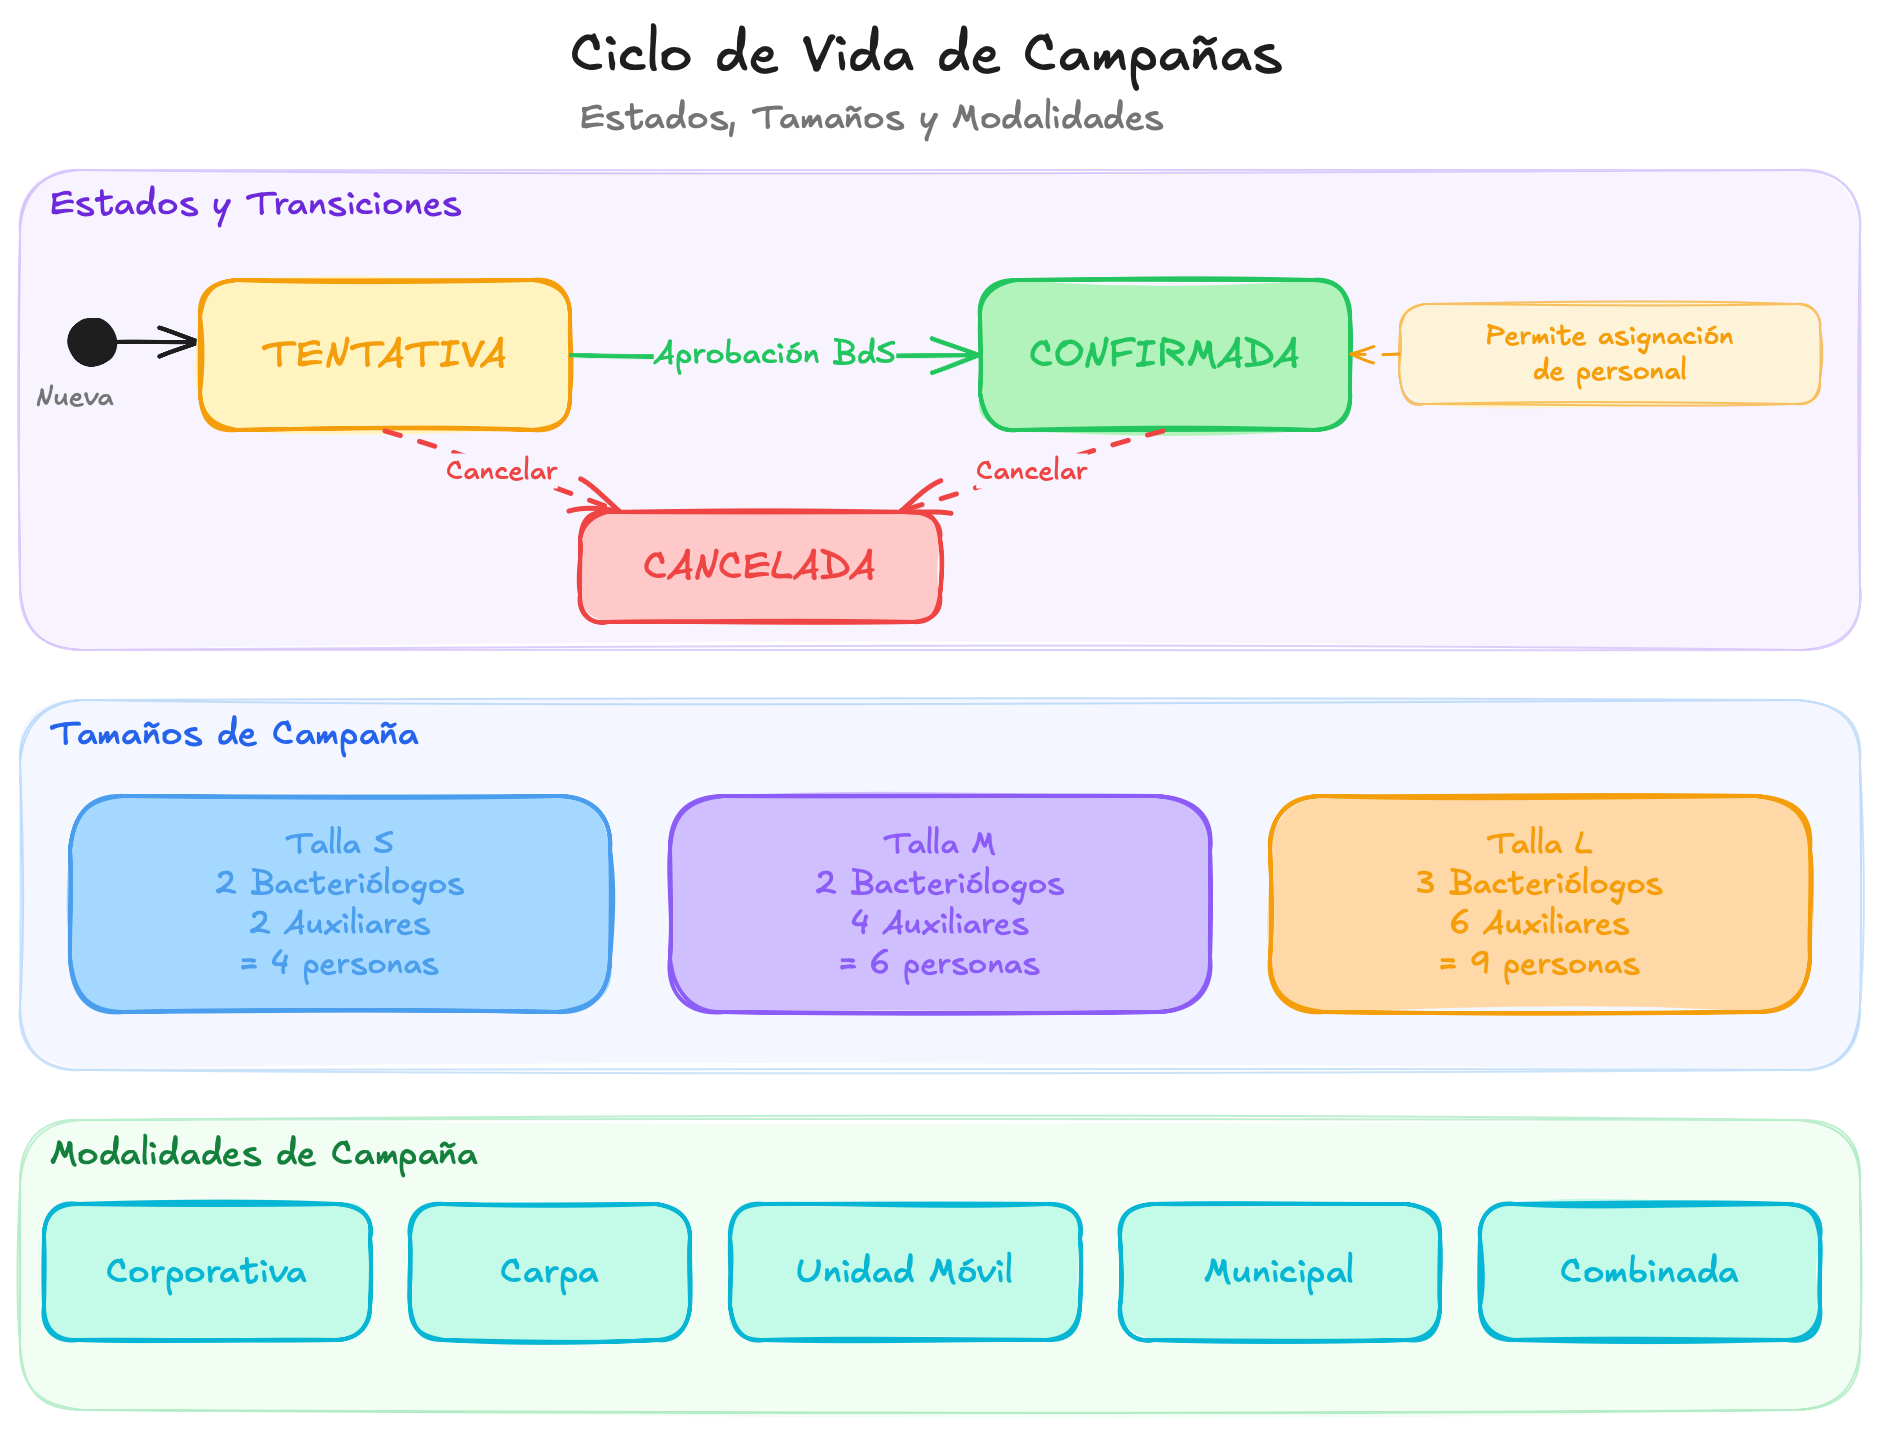
\includegraphics[width=0.92\textwidth]{Untitled-2026-02-11-1419.png}
\caption{Ciclo de vida de campañas: estados, transiciones, tamaños (S/M/L) y modalidades}
\label{fig:ciclo-vida-campanas}
\end{figure}

\subsection{Coordinador de Campaña (Designaci\'{o}n por Campaña)}

El coordinador de campaña \textbf{no es un rol fijo} del sistema. Es una \textbf{responsabilidad asignada por campaña}:

\begin{itemize}[leftmargin=2em]
    \item Al crear o editar una campaña, Banco de Sangre \textbf{designa a una persona del equipo asignado como coordinador} de esa campaña espec\'{i}fica.
    \item Esta designaci\'{o}n le habilita \textbf{permisos temporales} para esa campaña: registrar los tiempos reales de la l\'{i}nea de tiempo y observaciones de campo.
    \item Un empleado puede ser coordinador de una campaña y personal operativo en otra.
    \item El coordinador var\'{i}a de campaña en campaña; no es siempre la misma persona.
\end{itemize}

\subsubsection{L\'{i}nea de Tiempo de Campaña (Trazabilidad de Horas)}

Es fundamental registrar \textbf{todas las actividades de la l\'{i}nea de tiempo} de cada campaña para tener trazabilidad completa. El coordinador de campaña registra los siguientes momentos:

\begin{enumerate}[leftmargin=2em]
    \item \textbf{Hora de salida de sede:} Momento en que el equipo parte de la sede principal.
    \item \textbf{Hora de llegada al punto:} Llegada al lugar de la campaña.
    \item \textbf{Hora de inicio de campaña:} Inicio de la atenci\'{o}n a donantes.
    \item \textbf{Hora de salida a almuerzo:} Inicio del receso de almuerzo.
    \item \textbf{Hora de regreso de almuerzo:} Finalizaci\'{o}n del receso de almuerzo.
    \item \textbf{Hora de finalizaci\'{o}n de campaña:} Fin de la atenci\'{o}n a donantes.
    \item \textbf{Hora de recogida:} Momento en que se recoge al equipo y material.
    \item \textbf{Hora de llegada a sede:} Regreso del equipo a la sede principal.
    \item \textbf{Hora de salida de sede (fin):} Momento en que el personal termina su jornada y sale de sede.
\end{enumerate}

\textbf{Nota:} Estos registros permiten calcular con precisi\'{o}n las horas reales trabajadas, tiempos de desplazamiento y tiempos muertos para cada campaña.

% ══════════════════════════════════════════════════════════════
\section{Perfiles de Personal}
% ══════════════════════════════════════════════════════════════

\subsection{Tipos de Perfil}

\begin{table}[h!]
\centering
\begin{tabularx}{\textwidth}{|l|l|X|}
\hline
\textbf{Perfil} & \textbf{Rol} & \textbf{Descripci\'{o}n} \\
\hline
Bacteri\'{o}logo & Operativo & Profesional responsable del proceso de extracci\'{o}n y manejo de hemocomponentes. Participa en campañas seg\'{u}n su \'{a}rea de entrenamiento. \\
\hline
M\'{e}dico & Operativo & Profesional m\'{e}dico que atiende a donantes. Se asigna seg\'{u}n necesidad espec\'{i}fica de cada campaña. \\
\hline
T\'{e}cnico Operativo & Operativo & Auxiliar de enfermer\'{i}a. Apoya en el proceso de flebotom\'{i}a, atenci\'{o}n al donante y log\'{i}stica operativa de la campaña. \\
\hline
T\'{e}cnico Administrativo & Administrativo/Operativo & Personal administrativo que comenzar\'{a} a realizar turnos: completo, noche y posturno. Se incluir\'{a}n 2 t\'{e}cnicos administrativos y 2 t\'{e}cnicos operativos en estos turnos rotativos. \\
\hline
\end{tabularx}
\caption{Perfiles de personal del Banco de Sangre}
\end{table}

\subsection{\'{A}reas de Trabajo}

No todo el personal puede participar en todas las campañas. La capacidad de cada persona depende de su experiencia y experticia en las diferentes \'{a}reas.

\begin{itemize}[leftmargin=2em]
    \item El sistema tiene un \textbf{cat\'{a}logo de \'{a}reas de trabajo} disponibles (configurable por el administrador).
    \item Los \textbf{administradores} asignan a cada empleado una o m\'{a}s \'{a}reas en las que puede trabajar.
    \item Un empleado puede estar habilitado en \textbf{una, varias o todas} las \'{a}reas, seg\'{u}n su experiencia y experticia.
    \item Esta asignaci\'{o}n es \textbf{totalmente editable}: se pueden agregar o quitar \'{a}reas a un empleado en cualquier momento.
    \item Al momento de asignar personal a una campaña, el sistema \textbf{solo muestra personal habilitado} para el \'{a}rea requerida.
    \item No se manejan certificaciones ni documentos adjuntos; la habilitaci\'{o}n es una selecci\'{o}n directa del administrador.
\end{itemize}

\subsection{Turnos de T\'{e}cnicos Administrativos}

Los t\'{e}cnicos administrativos comenzar\'{a}n a rotar en tres tipos de turno:

\begin{table}[h!]
\centering
\begin{tabularx}{\textwidth}{|l|X|}
\hline
\textbf{Turno} & \textbf{Descripci\'{o}n} \\
\hline
Completo & Jornada diurna completa \\
\hline
Noche & Turno nocturno \\
\hline
Posturno & D\'{i}a de descanso posterior al turno nocturno \\
\hline
\end{tabularx}
\caption{Tipos de turno para t\'{e}cnicos administrativos}
\end{table}

Se incluir\'{a}n en esta rotaci\'{o}n: 2 t\'{e}cnicos administrativos + 2 t\'{e}cnicos operativos.

% ══════════════════════════════════════════════════════════════
\section{Programaci\'{o}n: Sede y Campañas}
% ══════════════════════════════════════════════════════════════

El sistema gestiona \textbf{dos flujos de programaci\'{o}n} sobre el mismo pool de personal. Las horas de ambos flujos se suman para el c\'{o}mputo semanal de cada empleado.

\subsection{Flujo 1: Turnos en Sede Principal}

El personal del Banco de Sangre cumple una \textbf{jornada laboral regular} en la sede principal. Este flujo permite:

\begin{itemize}[leftmargin=2em]
    \item Programar turnos semanales de cada empleado en sede (horario de entrada y salida).
    \item Registrar los tipos de turno: completo (diurno), noche y posturno.
    \item Llevar el control de horas regulares cumplidas en sede.
    \item Visualizar la ocupaci\'{o}n de personal en sede para saber qui\'{e}n est\'{a} disponible para campañas.
\end{itemize}

\textbf{Relaci\'{o}n con campañas:} Cuando un empleado es asignado a una campaña extramural, sus horas en sede se reducen o se reemplazan por las horas de campaña para esa jornada. El sistema debe reflejar esto autom\'{a}ticamente en el balance semanal.

\subsection{Flujo 2: Campañas Extramurales}

El personal se asigna a campañas fuera de sede seg\'{u}n su perfil, \'{a}rea de entrenamiento y disponibilidad. Este es el flujo descrito en detalle en las secciones de campañas, asignaci\'{o}n y reglas de negocio.

\subsection{C\'{o}mputo Integrado de Horas}

\begin{itemize}[leftmargin=2em]
    \item \textbf{Horas semanales} = horas en sede + horas en campaña.
    \item Si el total supera las 44 horas contratadas, el excedente se cuenta como \textbf{horas extras}.
    \item Si el total es menor a 44 horas (por ejemplo, porque se cancel\'{o} una campaña y no se reprogramaron horas en sede), el empleado \textbf{le debe horas} a la organizaci\'{o}n (se compensan en la semana siguiente).
    \item El calendario del sistema muestra ambos tipos de asignaci\'{o}n (sede y campaña) integrados en una sola vista por persona.
\end{itemize}

\begin{figure}[H]
\centering
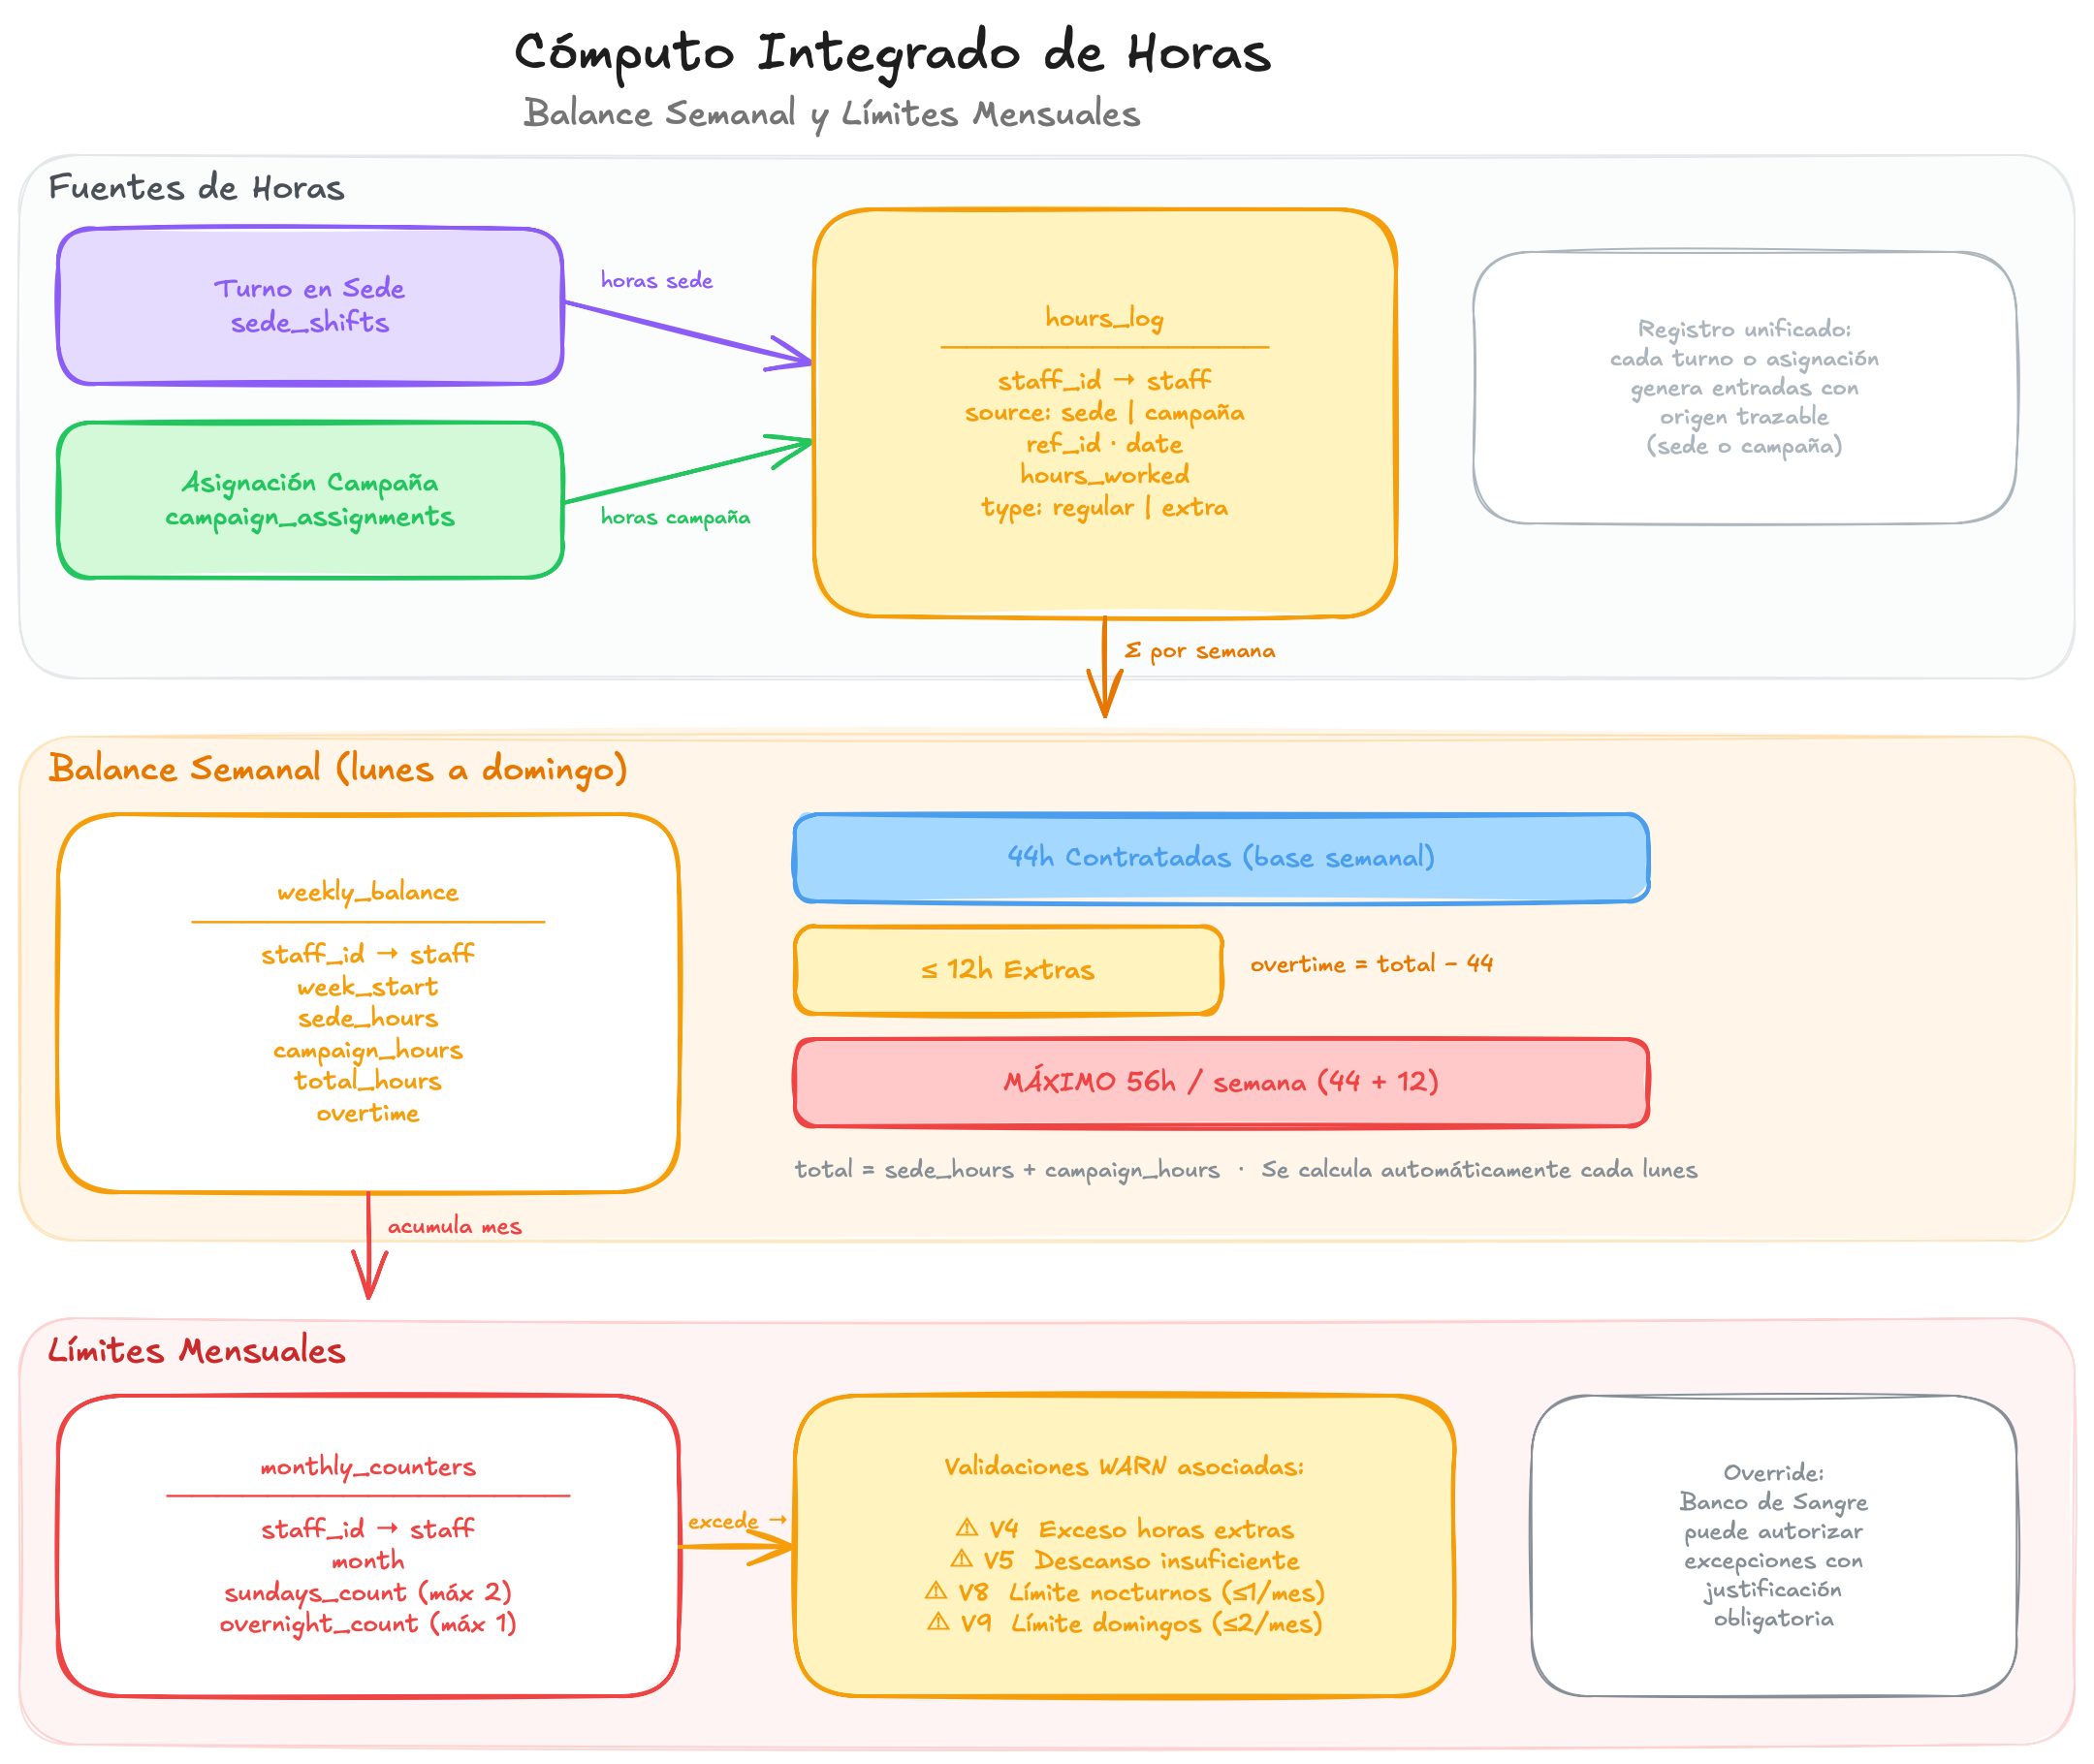
\includegraphics[width=\textwidth]{Untitled-2026-02-11-1419-8.png}
\caption{C\'{o}mputo integrado de horas: balance semanal (44h + 12h extras) y l\'{i}mites mensuales}
\label{fig:computo-horas}
\end{figure}

% ══════════════════════════════════════════════════════════════
\section{Reglas de Negocio y Validaciones}
% ══════════════════════════════════════════════════════════════

\subsection{Reglas Laborales Semanales}

Las siguientes reglas se configuran como \textbf{par\'{a}metros del sistema} (no est\'{a}n codificadas en duro), permitiendo ajustarlas ante cambios normativos sin modificar el c\'{o}digo fuente.

\begin{table}[h!]
\centering
\begin{tabularx}{\textwidth}{|l|X|c|}
\hline
\textbf{Par\'{a}metro} & \textbf{Descripci\'{o}n} & \textbf{Valor} \\
\hline
Jornada semanal & Horas ordinarias semanales por contrato & 44 horas \\
\hline
M\'{a}x. horas extras semanales & L\'{i}mite de horas extra por empleado por semana & 12 horas \\
\hline
M\'{a}x. horas por turno & Duraci\'{o}n m\'{a}xima de un turno continuo & 12 horas \\
\hline
Descanso m\'{i}nimo entre turnos & Horas de descanso obligatorio entre jornadas & 8 horas \\
\hline
\end{tabularx}
\caption{Par\'{a}metros laborales semanales configurables}
\end{table}

\subsection{Reglas Mensuales por Persona}

\begin{table}[h!]
\centering
\begin{tabularx}{\textwidth}{|l|X|c|}
\hline
\textbf{Par\'{a}metro} & \textbf{Descripci\'{o}n} & \textbf{Valor} \\
\hline
M\'{a}x. domingos por mes & N\'{u}mero m\'{a}ximo de domingos trabajados por empleado al mes & 2 \\
\hline
M\'{a}x. pernoctas por mes & N\'{u}mero m\'{a}ximo de pernoctas por empleado al mes & 1 \\
\hline
\end{tabularx}
\caption{Par\'{a}metros mensuales configurables}
\end{table}

\textbf{Restricciones de domingos:}
\begin{itemize}[leftmargin=2em]
    \item \textbf{Para Comercial:} Solo pueden programar campañas \textbf{m\'{a}ximo dos domingos al mes} en total (restricci\'{o}n a nivel de programaci\'{o}n de campañas).
    \item \textbf{Para el personal:} El sistema debe generar una \textbf{alerta} cuando un empleado haya trabajado dos domingos en el mes, impidiendo asignarlo a un tercer domingo.
\end{itemize}

\subsection{Reglas de Municipios y Pernoctas}

Cuando el personal se desplaza a \textbf{municipios diferentes} a la sede principal, aplican restricciones adicionales:

\begin{itemize}[leftmargin=2em]
    \item \textbf{D\'{i}a anterior a campaña municipal:} No se le deben programar campañas el d\'{i}a anterior. Si tiene jornada regular ese d\'{i}a, debe terminar \textbf{m\'{a}ximo a las 5:00 PM}.
    \item \textbf{D\'{i}a anterior a pernocta:} Misma restricci\'{o}n --- no programar campañas el d\'{i}a previo; jornada regular m\'{a}ximo hasta las 5:00 PM.
    \item El sistema debe \textbf{validar autom\'{a}ticamente} estas restricciones al momento de asignar personal a campañas municipales o con pernocta.
\end{itemize}

\subsection{Reglas de Asignaci\'{o}n}

\begin{itemize}[leftmargin=2em]
    \item No se puede asignar personal a dos actividades que se superpongan en horario.
    \item No se puede asignar personal que no est\'{e} capacitado para el \'{a}rea requerida por la campaña.
    \item El sistema debe \textbf{bloquear} asignaciones que violen l\'{i}mites duros (superposici\'{o}n, turno mayor a 12h, \'{a}rea no habilitada).
    \item El sistema debe \textbf{advertir} sobre l\'{i}mites blandos (proximidad al l\'{i}mite de horas extras, l\'{i}mite de domingos/pernoctas mensuales, descanso insuficiente, restricci\'{o}n de municipio).
    \item Las campañas requieren perfiles espec\'{i}ficos seg\'{u}n su tamaño: S (1+2), S+ (1+3), M (2+4), L (3+6).
    \item El personal cumple su \textbf{horario laboral normal} (intramural) adem\'{a}s de campañas; ambas jornadas cuentan para el c\'{o}mputo de horas.
\end{itemize}

\subsection{Calculadora de Horas y Balance Semanal}

\begin{enumerate}[leftmargin=2em]
    \item Obtener horas contratadas del empleado (por defecto: 44 horas semanales).
    \item Consultar todos los registros de horas de la semana (regulares + campañas + turnos).
    \item \textbf{Total} = horas regulares + horas de campaña + horas de turno.
    \item \textbf{Horas extras} = m\'{a}ximo(0, total $-$ 44).
    \item \textbf{Balance} = total $-$ 44:
    \begin{itemize}
        \item Si balance = 0: cumpli\'{o}.
        \item Si balance $>$ 0: tiene horas extras.
        \item Si balance $<$ 0: el empleado debe horas a la organizaci\'{o}n (se compensan la semana siguiente).
    \end{itemize}
    \item \textbf{Saldo arrastrado} = balance de la semana anterior que no se ha compensado.
    \item \textbf{Horas extras restantes} = m\'{a}ximo(0, 12 $-$ horas extras acumuladas).
\end{enumerate}

\subsection{Proyecci\'{o}n de Impacto}

Antes de confirmar una asignaci\'{o}n, el sistema calcula:
\begin{itemize}[leftmargin=2em]
    \item Horas extras \textbf{actuales} del empleado en la semana.
    \item Horas que \textbf{agregar\'{i}a} la nueva asignaci\'{o}n (desde hora inicio hasta hora estimada fin).
    \item Horas extras \textbf{proyectadas} = actuales + nuevas.
    \item Si proyectadas $>$ 12: muestra advertencia con el excedente.
    \item Si la campaña es en \textbf{domingo}: verifica conteo mensual (m\'{a}x. 2).
    \item Si la campaña requiere \textbf{pernocta}: verifica conteo mensual (m\'{a}x. 1).
\end{itemize}

\subsection{Detector de Conflictos (9 Validaciones)}

\begin{table}[h!]
\centering
\small
\begin{tabularx}{\textwidth}{|c|l|c|X|}
\hline
\textbf{\#} & \textbf{Conflicto} & \textbf{Severidad} & \textbf{Descripci\'{o}n} \\
\hline
1 & Superposici\'{o}n horaria & BLOQUEA & Ya asignado a otra actividad en el mismo horario \\
\hline
2 & Turno excesivo & BLOQUEA & El turno supera 12 horas \\
\hline
3 & \'{A}rea no habilitada & BLOQUEA & No est\'{a} capacitado para el \'{a}rea de la campaña \\
\hline
4 & Exceso horas extras & ADVIERTE & Excedr\'{i}a las 12 horas extras semanales \\
\hline
5 & No disponible & ADVIERTE & Marcado como no disponible \\
\hline
6 & Descanso insuficiente & ADVIERTE & Menos de 8 horas entre turnos \\
\hline
7 & L\'{i}mite domingos & ADVIERTE & Ya trabaj\'{o} 2 domingos este mes \\
\hline
8 & L\'{i}mite pernoctas & ADVIERTE & Ya tuvo 1 pernocta este mes \\
\hline
9 & Restricci\'{o}n municipio & ADVIERTE & Tiene actividad el d\'{i}a anterior que termina despu\'{e}s de las 5pm \\
\hline
\end{tabularx}
\caption{Validaciones del detector de conflictos}
\end{table}

\begin{figure}[H]
\centering
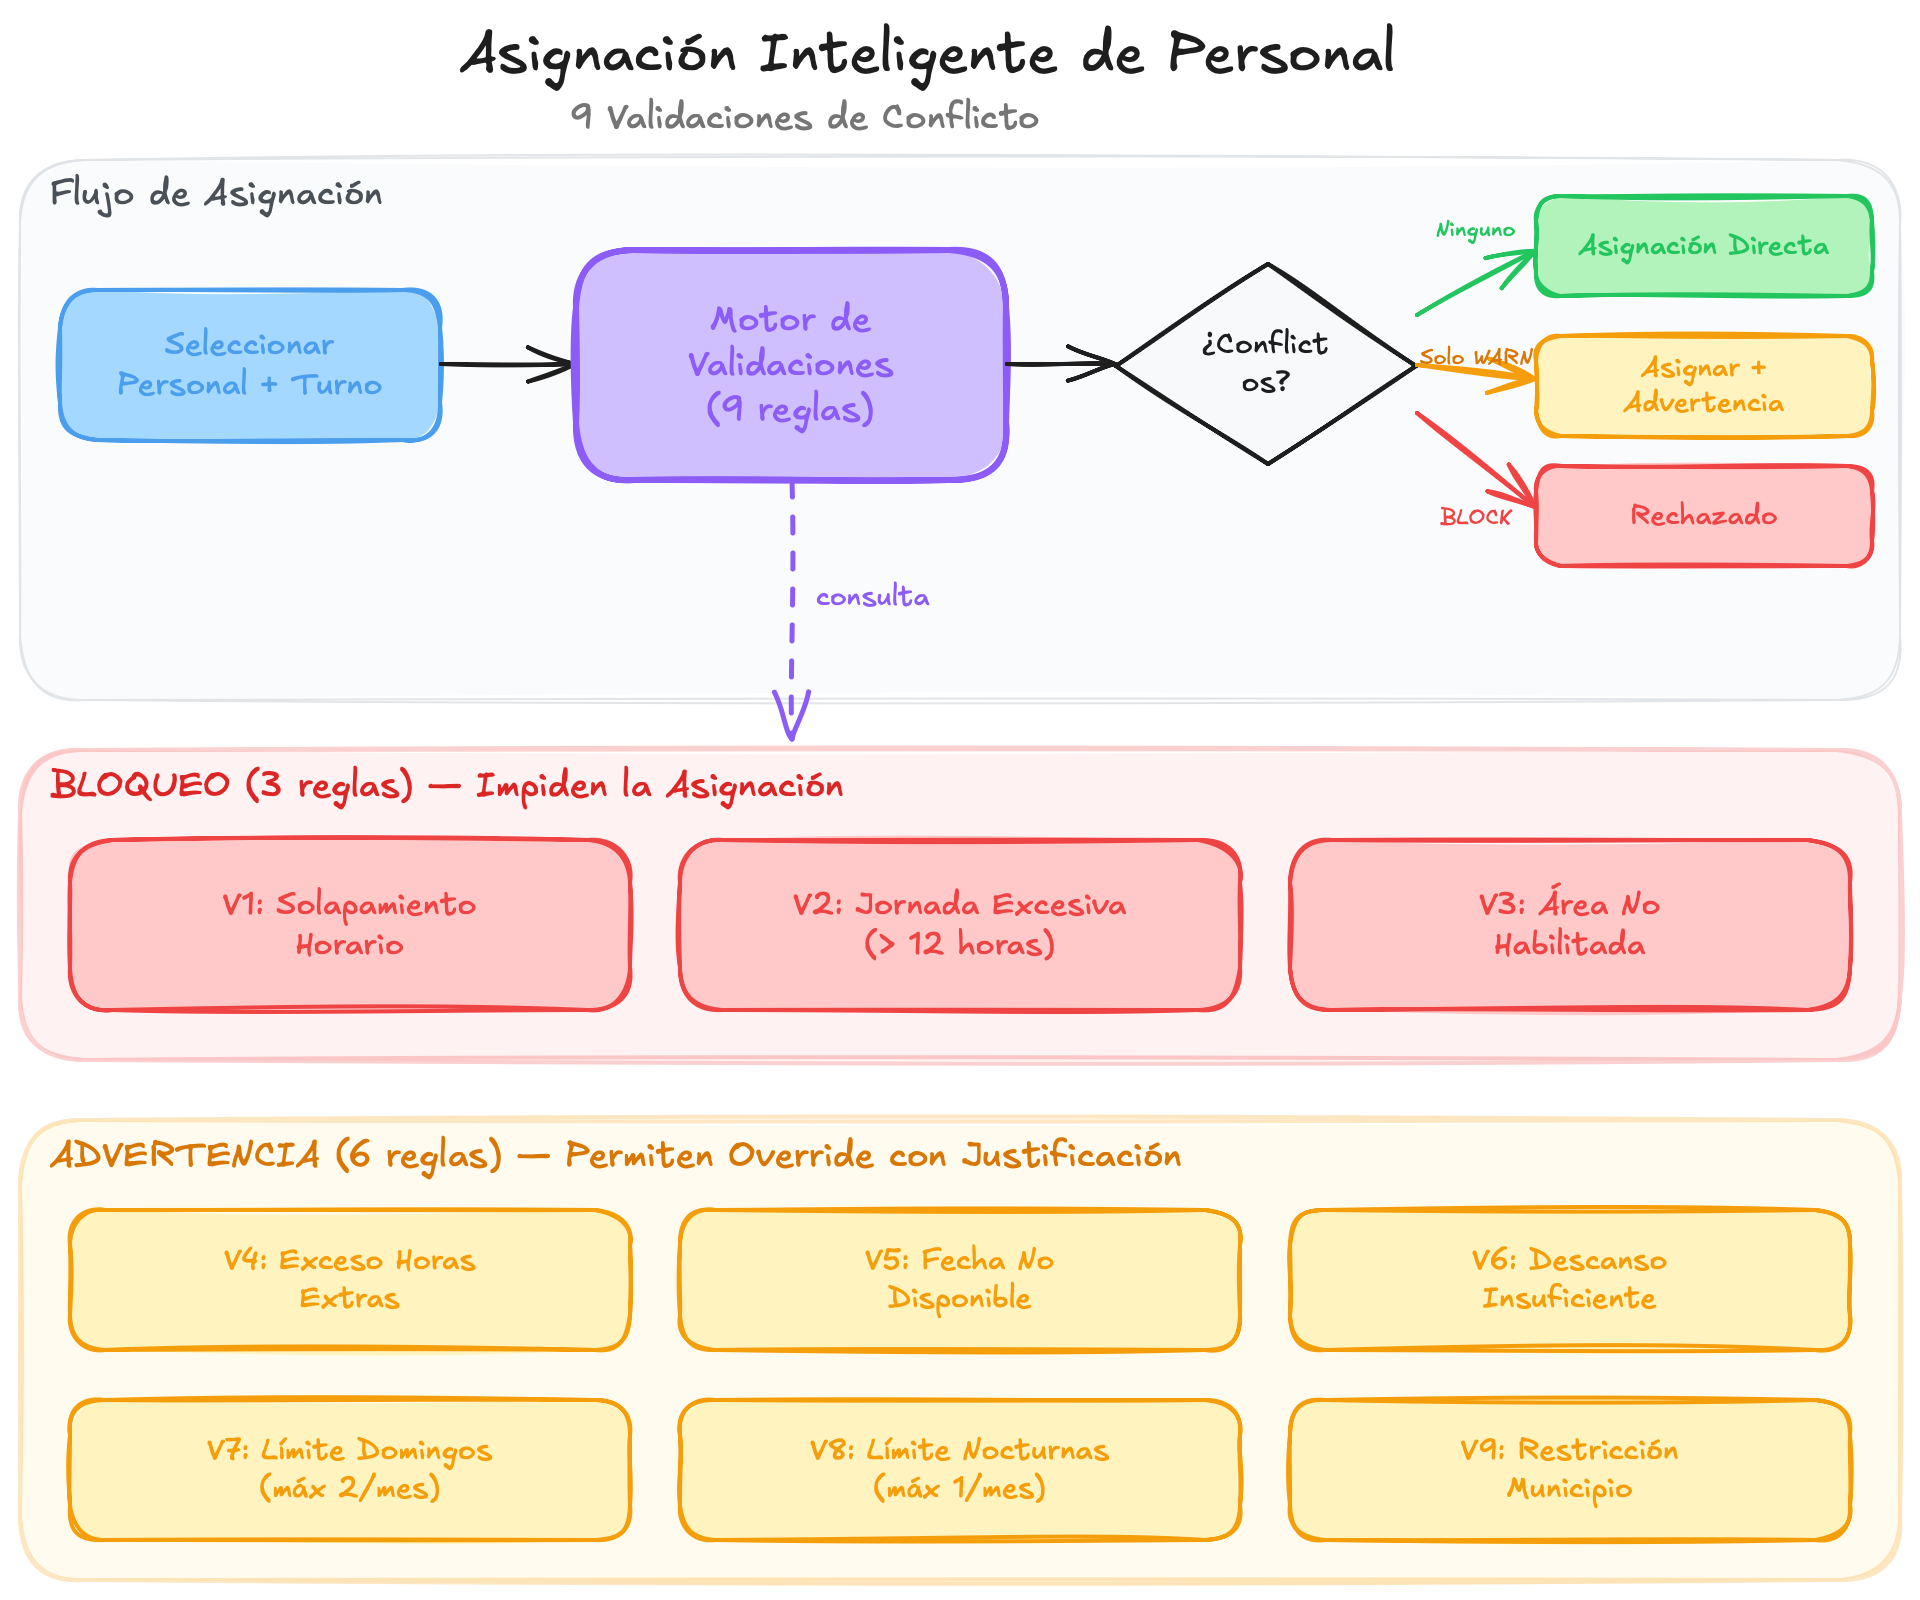
\includegraphics[width=0.85\textwidth]{Untitled-2026-02-11-1419-3.png}
\caption{Asignaci\'{o}n inteligente de personal: motor de 9 validaciones (3 BLOCK + 6 WARN)}
\label{fig:asignacion-inteligente}
\end{figure}

\subsection{Motor de Disponibilidad}

Para cada candidato a una campaña, el sistema calcula un \textbf{puntaje de disponibilidad}:

\begin{itemize}[leftmargin=2em]
    \item Base: 100 puntos.
    \item $-$30 si est\'{a} cerca del l\'{i}mite de horas extras (advertencia de proximidad).
    \item $-$50 si est\'{a} marcado como no disponible.
    \item $-$20 si tiene menos de 4 horas extras restantes.
    \item $-$15 si ya tiene 1 domingo trabajado en el mes (para campañas dominicales).
    \item $-$25 si tiene restricci\'{o}n de municipio el d\'{i}a anterior.
    \item Los candidatos se ordenan de mayor a menor puntaje.
    \item Los candidatos bloqueados (BLOQUEA) se muestran al final, deshabilitados.
\end{itemize}

% ══════════════════════════════════════════════════════════════
\section{Integraciones Externas}
% ══════════════════════════════════════════════════════════════

\subsection{Flujo CRM $\rightarrow$ Excel $\rightarrow$ Plataforma}

El equipo comercial \textbf{no recibe solicitudes de campañas}: las busca activamente (es un proceso de venta, ya que implica gestionar aproximadamente una hora por empleado de la empresa cliente). El flujo es:

\begin{enumerate}[leftmargin=2em]
    \item \textbf{Comercial} gestiona y concreta campañas con empresas/organizaciones.
    \item Registra la campaña en el \textbf{CRM de la empresa}.
    \item Exporta la informaci\'{o}n del CRM a un \textbf{archivo Excel} con los datos de la campaña.
    \item El archivo Excel se \textbf{carga semanalmente a la plataforma}. Las campañas se crean en estado \textbf{tentativa}.
    \item \textbf{Comercial} revisa y \textbf{confirma} las campañas en la plataforma (cambia estado a \textbf{confirmada}).
    \item Banco de Sangre \textbf{asigna el personal} a las campañas confirmadas, usando las reglas y validaciones del sistema.
    \item Comercial puede \textbf{consultar en la plataforma} los datos de personal asignado a cada campaña.
\end{enumerate}

\begin{figure}[H]
\centering
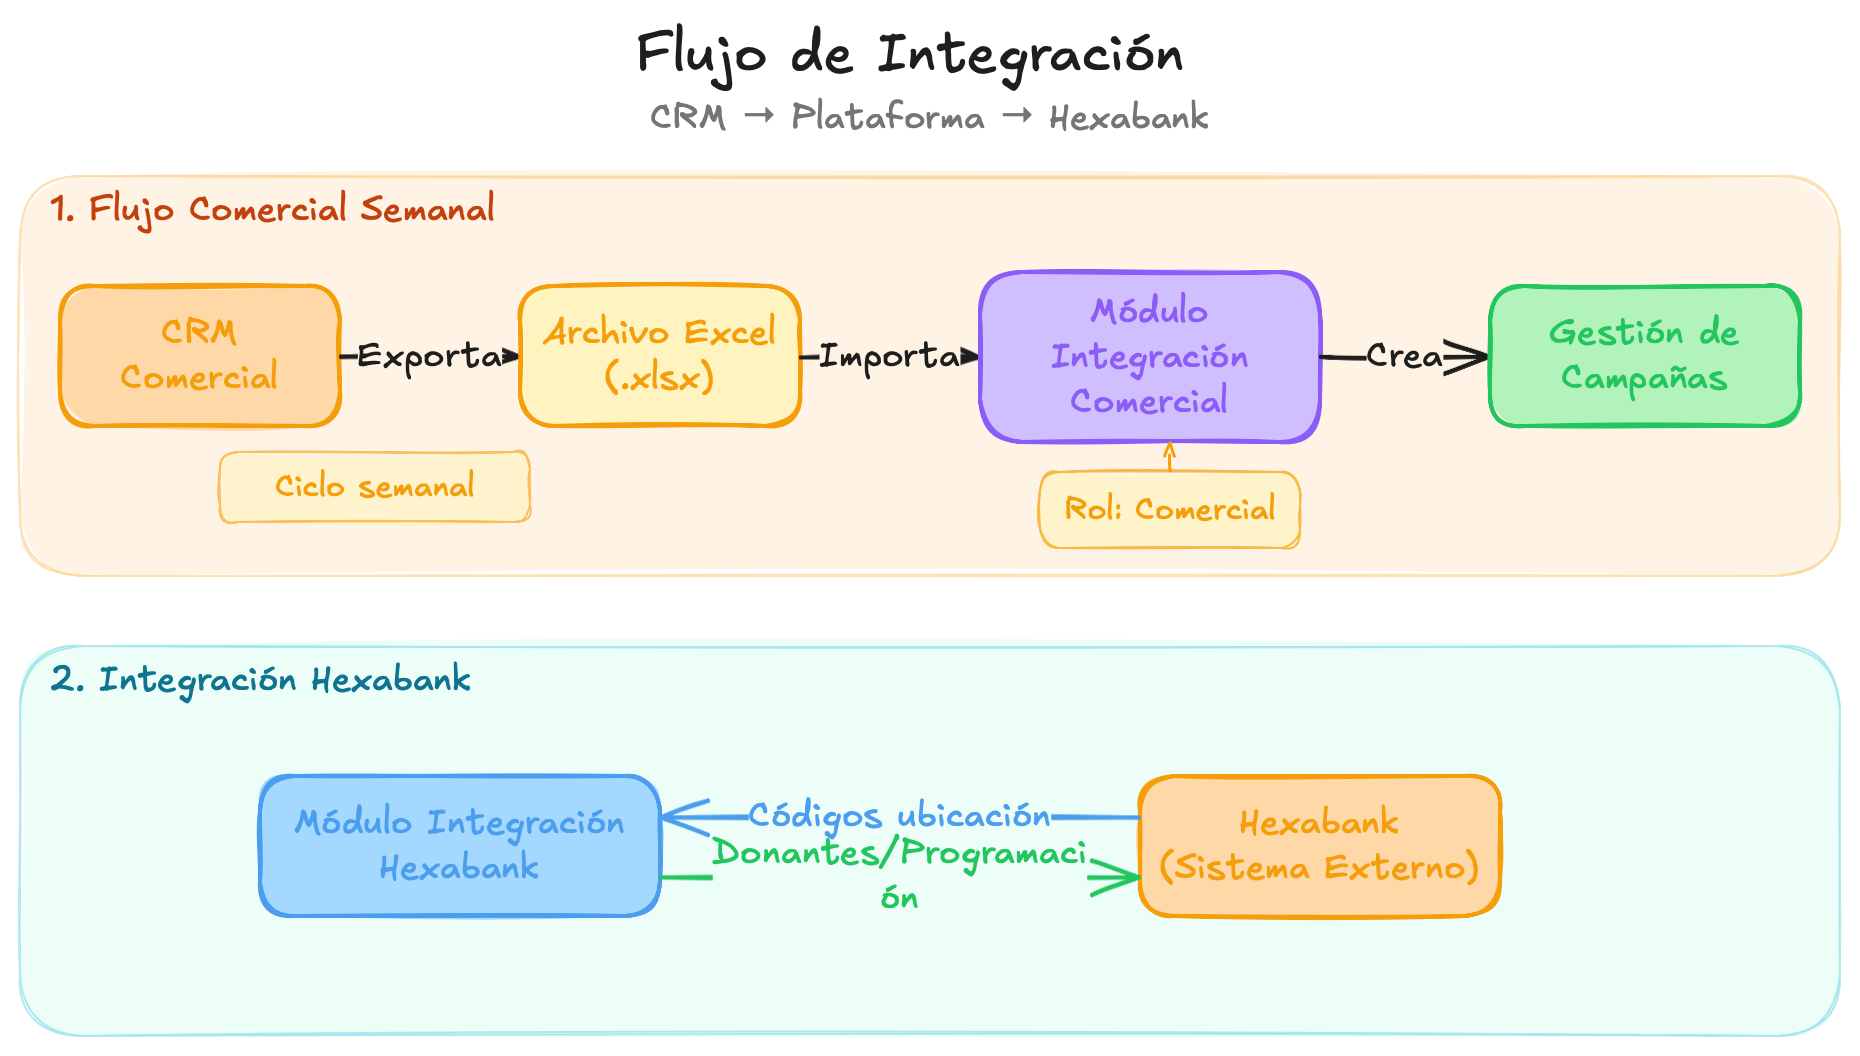
\includegraphics[width=0.88\textwidth]{Untitled-2026-02-11-1419-4.png}
\caption{Flujo de integraci\'{o}n: CRM $\rightarrow$ Excel $\rightarrow$ Plataforma $\rightarrow$ Hexabank}
\label{fig:flujo-integracion}
\end{figure}

\subsection{Datos que Importa Comercial (desde CRM/Excel)}

\begin{table}[h!]
\centering
\begin{tabularx}{\textwidth}{|l|X|}
\hline
\textbf{Campo} & \textbf{Descripci\'{o}n} \\
\hline
C\'{o}digo & Identificador \'{u}nico de la campaña (del CRM) \\
\hline
Nombre de la empresa & Empresa u organizaci\'{o}n donde se realizar\'{a} la campaña \\
\hline
Municipio & Municipio donde se realizar\'{a} \\
\hline
Mix (tamaño) & Tipo de campaña: S, M o L \\
\hline
Fecha & Fecha programada \\
\hline
Modalidad & Corporativa, carpa, unidad m\'{o}vil, municipal, combinada \\
\hline
Observaciones & Campo libre para notas adicionales \\
\hline
\end{tabularx}
\caption{Campos del archivo Excel de importaci\'{o}n desde CRM}
\end{table}

\subsection{Datos que Consulta Comercial (desde la Plataforma)}

Una vez que Banco de Sangre asigna el personal a la campaña (registrada por Comercial), Comercial necesita ver:

\begin{itemize}[leftmargin=2em]
    \item C\'{o}digo y nombre de la empresa.
    \item Municipio, fecha y modalidad.
    \item \textbf{Personal asignado:} nombres completos, n\'{u}mero de c\'{e}dula y cargo de cada persona.
    \item Estado de la campaña (tentativa, confirmada, cancelada).
\end{itemize}

\subsection{Integraci\'{o}n con Hexabank}

Hexabank es el sistema de gesti\'{o}n del Banco de Sangre del cual se requieren dos datos clave:

\begin{itemize}[leftmargin=2em]
    \item \textbf{C\'{o}digo de lugar:} Cada punto de recolecci\'{o}n tiene un c\'{o}digo en Hexabank. La plataforma debe permitir \textbf{relacionar cada campaña con su c\'{o}digo de lugar de Hexabank}.
    \item \textbf{Datos de donantes:} Horas y fechas de donaci\'{o}n. Estos datos se toman desde Hexabank para an\'{a}lisis y seguimiento.
\end{itemize}

\textbf{Nota:} En la primera fase, esta integraci\'{o}n puede ser manual (campo de texto para el c\'{o}digo). En fases posteriores se puede automatizar v\'{i}a API si Hexabank lo permite.

\subsection{Migraci\'{o}n de Directorio de Contactos}

Comercial requiere migrar su \textbf{base de datos de directorio} (contactos de empresas, organizaciones, responsables) a la plataforma para centralizar la gesti\'{o}n de contactos y facilitar la creaci\'{o}n de campañas.

% ══════════════════════════════════════════════════════════════
\section{Roles y Permisos}
% ══════════════════════════════════════════════════════════════

El sistema define \textbf{cuatro roles fijos} con permisos diferenciados, m\'{a}s una \textbf{designaci\'{o}n por campaña} (coordinador):

\begin{table}[h!]
\centering
\small
\begin{tabularx}{\textwidth}{|X|c|c|c|c|}
\hline
\textbf{Funcionalidad} & \textbf{Admin} & \textbf{B. Sangre} & \textbf{Comercial} & \textbf{Operativo} \\
\hline
Dashboard general & S\'{i} & S\'{i} & S\'{i} & S\'{i} (personal) \\
\hline
Crear/editar personal & S\'{i} & S\'{i} & --- & --- \\
\hline
Ver directorio personal & S\'{i} & S\'{i} & --- & --- \\
\hline
Programar turnos en sede & S\'{i} & S\'{i} & --- & --- \\
\hline
Crear/editar campañas & S\'{i} & --- & S\'{i} & --- \\
\hline
Confirmar/cancelar campañas & S\'{i} & --- & S\'{i} & --- \\
\hline
Ver campañas & S\'{i} & S\'{i} & S\'{i} & Solo asignadas \\
\hline
Asignar personal & S\'{i} & S\'{i} & --- & --- \\
\hline
Designar coordinador & S\'{i} & S\'{i} & --- & --- \\
\hline
Cargar Excel CRM & S\'{i} & S\'{i} & S\'{i} & --- \\
\hline
Ver personal asignado & S\'{i} & S\'{i} & S\'{i} (nombre, CC, cargo) & --- \\
\hline
Registrar hora real* & S\'{i} & S\'{i} & --- & Solo si es coord. \\
\hline
Ver disponibilidad & S\'{i} & S\'{i} & S\'{i} (resumen) & Solo propia \\
\hline
Reportes de horas & S\'{i} & S\'{i} & --- & Solo propias \\
\hline
Reportes de campañas & S\'{i} & S\'{i} & S\'{i} & --- \\
\hline
Configuraci\'{o}n sistema & S\'{i} & --- & --- & --- \\
\hline
\end{tabularx}
\caption{Matriz de permisos por rol (*el registro de hora real lo puede hacer cualquier persona designada como coordinador de esa campaña espec\'{i}fica)}
\end{table}

\begin{figure}[H]
\centering
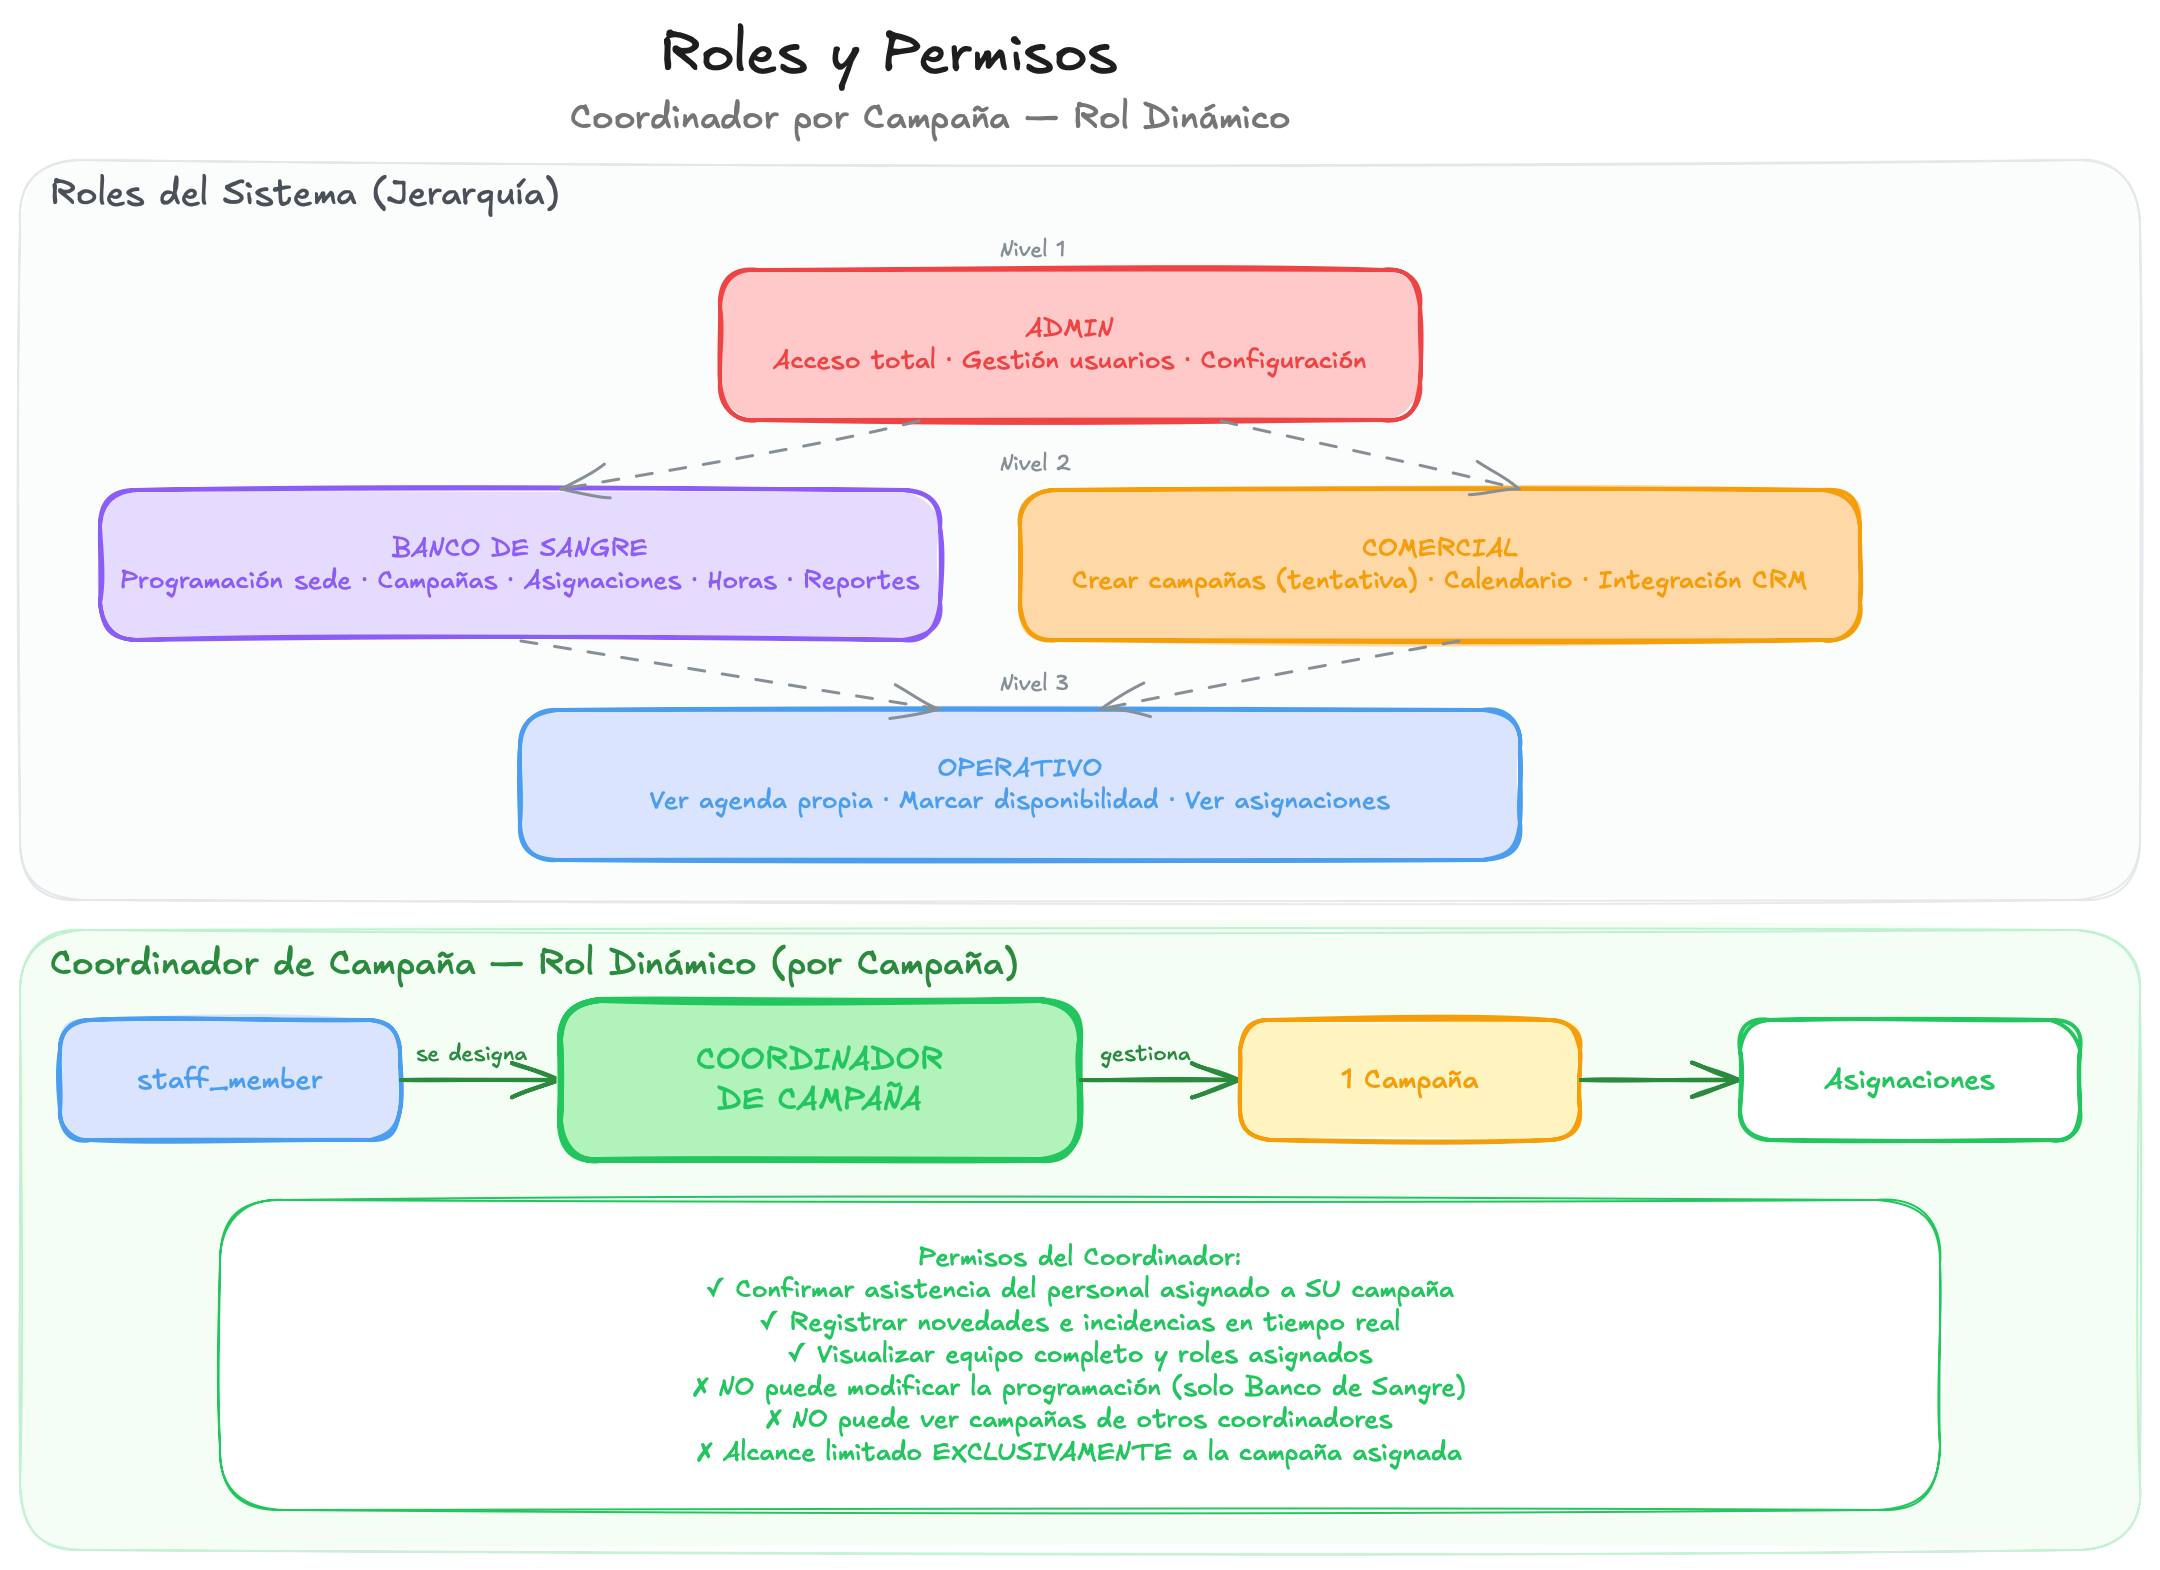
\includegraphics[width=0.92\textwidth]{Untitled-2026-02-11-1419-7.png}
\caption{Roles y permisos: jerarqu\'{i}a de 4 roles del sistema + coordinador de campaña (rol din\'{a}mico)}
\label{fig:roles-permisos}
\end{figure}

\textbf{Roles fijos del sistema:}
\begin{itemize}[leftmargin=2em]
    \item \textbf{Admin:} Control total del sistema, configuraci\'{o}n y gesti\'{o}n de usuarios.
    \item \textbf{Banco de Sangre:} Programa turnos en sede, asigna personal a campañas confirmadas, designa coordinadores, gestiona horas y programaci\'{o}n.
    \item \textbf{Comercial:} Carga campañas desde CRM (Excel), confirma y cancela campañas, consulta personal asignado (nombre, c\'{e}dula, cargo), ve calendario de capacidad.
    \item \textbf{Operativo:} Ve su propio calendario (sede + campañas), horas, balance semanal y asignaciones. Reporta disponibilidad.
\end{itemize}

\textbf{Designaci\'{o}n por campaña:}
\begin{itemize}[leftmargin=2em]
    \item \textbf{Coordinador de campaña:} No es un rol del sistema sino una \textbf{responsabilidad asignada por campaña} desde Banco de Sangre. La persona designada (que puede tener cualquier rol, generalmente Operativo) obtiene \textbf{permisos temporales} para registrar horas reales de llegada, finalizaci\'{o}n y observaciones de campo \textbf{solo para esa campaña espec\'{i}fica}. Var\'{i}a de campaña en campaña.
\end{itemize}

% ══════════════════════════════════════════════════════════════
\section{Flujos de Trabajo Principales}
% ══════════════════════════════════════════════════════════════

\subsection{Flujo 1: Carga y Confirmaci\'{o}n de Campañas (Comercial $\rightarrow$ Banco de Sangre)}

\begin{enumerate}[leftmargin=2em]
    \item \textbf{Comercial} concreta campañas con empresas/organizaciones y las registra en el CRM.
    \item Semanalmente, exporta los datos del CRM a un archivo Excel.
    \item Sube el Excel a la plataforma (campos: c\'{o}digo, empresa, municipio, mix, fecha, modalidad, observaciones).
    \item El sistema valida los datos y crea las campañas en estado \textbf{tentativa}.
    \item \textbf{Comercial} revisa las campañas importadas, ajusta si es necesario y las \textbf{confirma} (estado pasa a \textbf{confirmada}).
    \item \textbf{Banco de Sangre} recibe las campañas confirmadas y procede con la \textbf{asignaci\'{o}n de personal} seg\'{u}n las reglas del sistema.
\end{enumerate}

\subsection{Flujo 2: Asignaci\'{o}n de Personal (Banco de Sangre)}

\begin{enumerate}[leftmargin=2em]
    \item Banco de Sangre abre una campaña confirmada.
    \item El sistema muestra los requerimientos seg\'{u}n el tamaño (ej: M = 2 bacteri\'{o}logos + 4 t\'{e}cnicos).
    \item Selecciona ``Asignar Personal''. El sistema muestra panel inteligente:
    \begin{itemize}
        \item Filtra por perfil requerido \textbf{y} \'{a}rea de entrenamiento habilitada.
        \item Excluye personal con conflictos de horario.
        \item Valida restricci\'{o}n de municipio (d\'{i}a anterior libre o max. 5pm).
        \item Valida l\'{i}mites mensuales (max. 2 domingos, max. 1 pernocta).
        \item Muestra balance semanal y horas extras restantes de cada candidato.
        \item Sem\'{a}foro: verde / amarillo / rojo.
    \end{itemize}
    \item Banco de Sangre selecciona personal. El sistema valida:
    \begin{itemize}
        \item \textbf{BLOQUEA} si hay superposici\'{o}n, turno excesivo o \'{a}rea no habilitada.
        \item \textbf{ADVIERTE} si se acerca al l\'{i}mite de extras, domingos o pernoctas.
    \end{itemize}
    \item Confirma asignaciones.
    \item \textbf{Designa coordinador:} De entre el personal asignado, selecciona a una persona como coordinador de esa campaña. Esto le habilita permisos para registrar horas reales.
    \item Comercial puede ver en la plataforma el personal asignado (nombre, c\'{e}dula, cargo).
\end{enumerate}

\subsection{Flujo 3: Programaci\'{o}n de Turnos en Sede (Banco de Sangre)}

\begin{enumerate}[leftmargin=2em]
    \item Banco de Sangre navega al m\'{o}dulo de ``Programaci\'{o}n en Sede''.
    \item Selecciona la semana a programar.
    \item Asigna turnos a cada empleado: d\'{i}a, tipo de turno (completo, noche, posturno), hora de inicio y fin.
    \item El sistema valida que no haya conflictos con campañas ya asignadas para ese d\'{i}a.
    \item Las horas de sede se reflejan autom\'{a}ticamente en el balance semanal de cada empleado.
    \item Si un empleado es asignado a una campaña extramural, su turno de sede para ese d\'{i}a se ajusta o reemplaza.
\end{enumerate}

\subsection{Flujo 4: Registro de Horas Reales (Coordinador de Campaña)}

\begin{enumerate}[leftmargin=2em]
    \item La campaña tiene hora de inicio programada y hora estimada de fin calculada.
    \item La persona designada como coordinador de esa campaña asiste a la jornada.
    \item Durante y al finalizar la campaña, el coordinador registra la \textbf{l\'{i}nea de tiempo completa}: hora de salida de sede, hora de llegada al punto, hora de inicio de campaña, horas de almuerzo, hora de finalizaci\'{o}n, hora de recogida, hora de llegada a sede y hora de salida de sede, junto con observaciones de campo.
    \item Solo tiene permiso para registrar datos de \textbf{esa campaña espec\'{i}fica} (no de otras).
    \item El sistema calcula las horas reales trabajadas a partir de la l\'{i}nea de tiempo y actualiza el balance semanal de cada persona asignada.
\end{enumerate}

\subsection{Flujo 5: Monitoreo Semanal de Horas y Balance}

\begin{enumerate}[leftmargin=2em]
    \item Admin/Banco de Sangre navega a ``Reporte de Horas''.
    \item Selecciona semana.
    \item Sistema muestra tabla:

    \small
    \begin{tabularx}{\textwidth}{|l|l|c|c|c|c|c|c|}
    \hline
    \textbf{Empleado} & \textbf{Perfil} & \textbf{Sede} & \textbf{Camp.} & \textbf{Total} & \textbf{Extras} & \textbf{\%} & \textbf{Balance} \\
    \hline
    J. P\'{e}rez & Bact. & 36h & 8h & 44h & 0h & 0\% & Cumpli\'{o} \\
    \hline
    M. L\'{o}pez & T\'{e}c.Op. & 44h & 14h & 58h & 14h & \textcolor{red}{117\%} & +14h extras \\
    \hline
    A. G\'{o}mez & T\'{e}c.Adm. & 38h & 0h & 38h & 0h & 0\% & Debe 6h \\
    \hline
    R. D\'{i}az & Bact. & 24h & 16h & 40h & 0h & 0\% & Debe 4h \\
    \hline
    \end{tabularx}
    \normalsize

    \item Filas codificadas por color seg\'{u}n porcentaje de l\'{i}mite.
    \item Balance: cumpli\'{o}, le deben horas, o debe horas (se compensa la semana siguiente).
    \item Bot\'{o}n de exportar a Excel.
\end{enumerate}

\subsection{Flujo 6: Vista Personal Operativo}

\begin{enumerate}[leftmargin=2em]
    \item Empleado inicia sesi\'{o}n y ve su dashboard personal.
    \item Ve en un \textbf{calendario integrado}: turnos en sede + campañas asignadas (pr\'{o}ximas 2 semanas).
    \item Ve resumen de horas de la semana: sede + campañas = total, balance acumulado.
    \item Ve contadores del mes: domingos trabajados (de 2) y pernoctas (de 1).
    \item Si fue designado coordinador de alguna campaña, ve un acceso directo para registrar horas reales.
    \item Puede marcar fechas como no disponible con motivo.
    \item Puede consultar hist\'{o}rico de campañas, turnos y horas.
\end{enumerate}

\subsection{Flujo 7: Cancelaci\'{o}n de Campaña}

\textbf{Responsable: Comercial} (es quien establece el contacto directo con la empresa).

\begin{enumerate}[leftmargin=2em]
    \item \textbf{Comercial} abre detalle de campaña y selecciona ``Cancelar''.
    \item Debe ingresar motivo de cancelaci\'{o}n (obligatorio).
    \item Sistema muestra personal afectado y horas que se liberar\'{a}n.
    \item Al confirmar: todas las asignaciones se anulan, estado cambia a \textit{cancelada}.
    \item Banco de Sangre es notificado de la cancelaci\'{o}n para ajustar la programaci\'{o}n del personal.
    \item Queda registrado en log de auditor\'{i}a.
\end{enumerate}

% ╔════════════════════════════════════════════════════════════╗
% ║            PARTE III — ARQUITECTURA T\'{E}CNICA              ║
% ╚════════════════════════════════════════════════════════════╝

% ══════════════════════════════════════════════════════════════
\section{Stack Tecnol\'{o}gico y Arquitectura}
% ══════════════════════════════════════════════════════════════

\subsection{Tecnolog\'{i}as Principales}

\begin{table}[h!]
\centering
\begin{tabularx}{\textwidth}{|l|l|X|}
\hline
\textbf{Capa} & \textbf{Tecnolog\'{i}a} & \textbf{Justificaci\'{o}n} \\
\hline
Framework & Next.js 15 (App Router) & Server Components, Server Actions, middleware RBAC \\
\hline
Lenguaje & TypeScript & Seguridad de tipos en todo el stack \\
\hline
ORM & Drizzle ORM & TypeScript-first, queries predecibles, migraciones \\
\hline
Base de datos & PostgreSQL 16 & Robusta para datos relacionales y scheduling \\
\hline
Autenticaci\'{o}n & Better Auth & Credenciales + RBAC integrado \\
\hline
UI & shadcn/ui + Tailwind CSS 4 & Componentes accesibles, personalizables \\
\hline
Formularios & React Hook Form + Zod & Validaci\'{o}n compartida cliente/servidor \\
\hline
Estado & TanStack Query v5 & Cache, actualizaciones optimistas \\
\hline
Calendario & FullCalendar v6 & Vistas d\'{i}a/semana/mes, drag-and-drop \\
\hline
Tablas & TanStack Table v8 & Ordenable, filtrable, paginada \\
\hline
Excel & SheetJS (xlsx) & Lectura y escritura de archivos .xlsx \\
\hline
Fechas & date-fns v3 & Manipulaci\'{o}n de fechas con timezone \\
\hline
Deployment & Docker + Docker Compose & Despliegue consistente \\
\hline
\end{tabularx}
\caption{Stack tecnol\'{o}gico del sistema}
\end{table}

\subsection{Decisiones de Arquitectura}

\begin{enumerate}[leftmargin=2em]
    \item \textbf{Better Auth sobre Auth.js}: Autenticaci\'{o}n por credenciales m\'{a}s simple y estable para una app interna sin necesidad de OAuth.
    \item \textbf{Drizzle sobre Prisma}: M\'{a}s cercano a SQL, queries predecibles, ideal para consultas complejas de scheduling y c\'{a}lculos de horas.
    \item \textbf{Server Actions como capa principal de datos}: Elimina la necesidad de una API REST separada. API routes solo para importaci\'{o}n/exportaci\'{o}n de archivos Excel.
    \item \textbf{Par\'{a}metros laborales en base de datos}: Permite ajustar reglas ante cambios normativos sin redesplegar c\'{o}digo.
    \item \textbf{Conflictos con severidades}: Distingue entre bloqueos duros (imposibles) y advertencias (requieren criterio humano).
    \item \textbf{Integraci\'{o}n CRM v\'{i}a Excel}: Soluci\'{o}n pragm\'{a}tica que no requiere acceso directo al CRM; la carga semanal cubre el flujo operativo.
\end{enumerate}

\subsection{Principio de Diseño: M\'{o}dulos Gen\'{e}ricos}

El sistema se estructura en \textbf{m\'{o}dulos gen\'{e}ricos} que no dependen del tipo de operaci\'{o}n espec\'{i}fica. Cada m\'{o}dulo opera sobre conceptos abstractos que se instancian seg\'{u}n el \'{a}rea:

\begin{table}[h!]
\centering
\begin{tabularx}{\textwidth}{|l|l|X|}
\hline
\textbf{Concepto Gen\'{e}rico} & \textbf{En Donaci\'{o}n de Sangre} & \textbf{En Otras \'{A}reas (futuro)} \\
\hline
Actividad & Campaña de donaci\'{o}n & Operativo APH, Capacitaci\'{o}n, Brigada \\
\hline
Personal & Bact., M\'{e}d., T\'{e}c.Op., T\'{e}c.Adm. & Param\'{e}dico, Instructor, Log\'{i}stico \\
\hline
\'{A}rea de trabajo & \'{A}reas de Banco de Sangre & \'{A}reas de APH, Gesti\'{o}n del Riesgo, etc. \\
\hline
Ubicaci\'{o}n & Punto de recolecci\'{o}n & Centro de acopio, Zona de desastre \\
\hline
Fuente externa & CRM Comercial + Hexabank & Otros sistemas por \'{a}rea \\
\hline
\end{tabularx}
\caption{Mapeo de conceptos gen\'{e}ricos a implementaciones espec\'{i}ficas}
\end{table}

\begin{figure}[H]
\centering
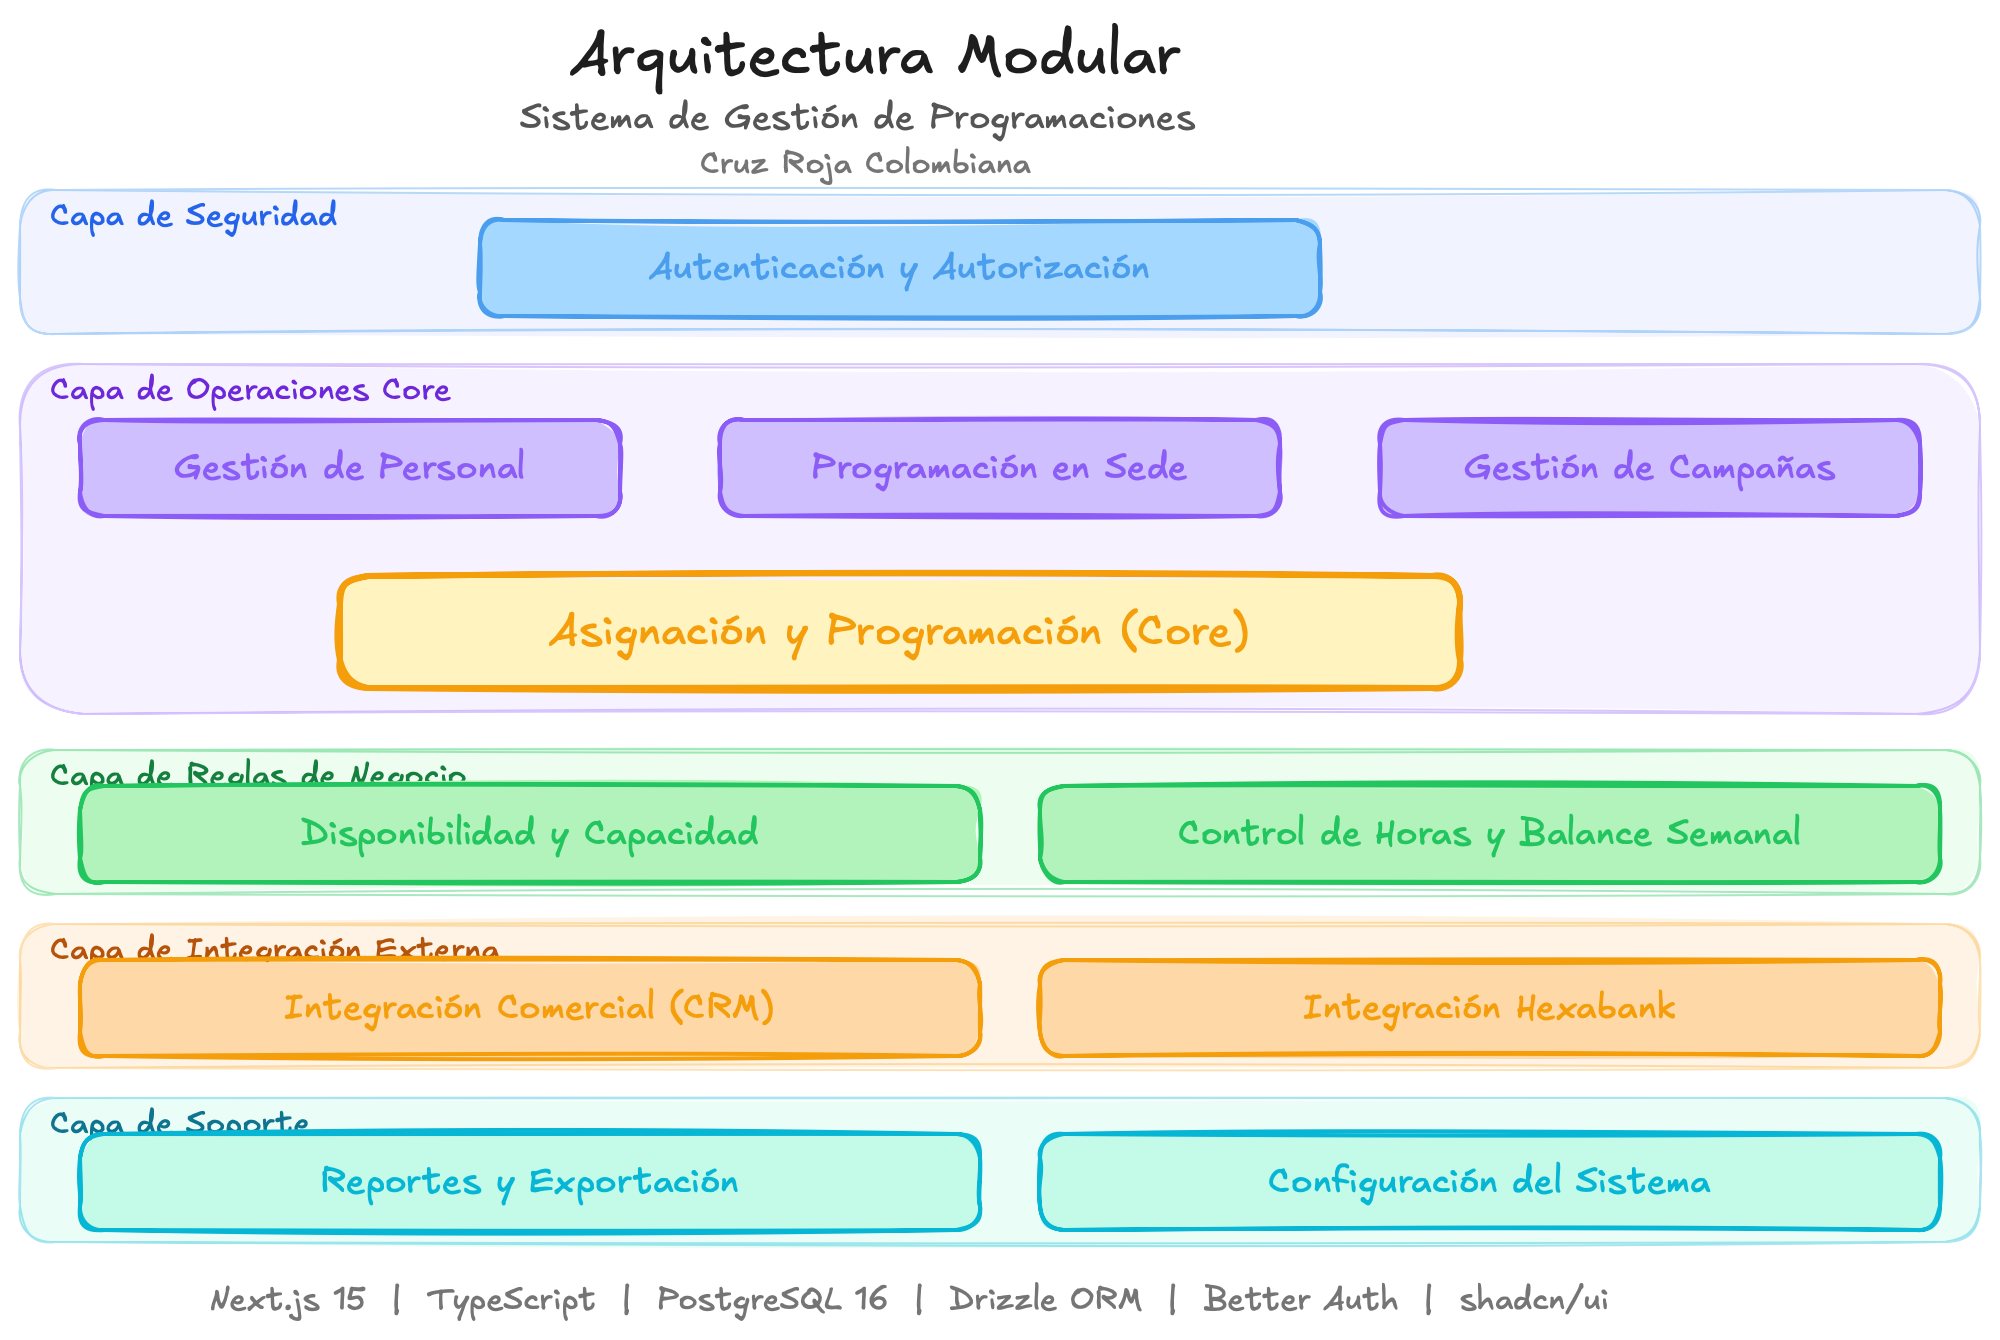
\includegraphics[width=0.92\textwidth]{Untitled-2026-02-11-1419-6.png}
\caption{Arquitectura modular: 11 m\'{o}dulos en 5 capas con stack tecnol\'{o}gico}
\label{fig:arquitectura-modular}
\end{figure}

\subsection{M\'{o}dulos del Sistema}

\subsubsection{M\'{o}dulo 1: Autenticaci\'{o}n y Autorizaci\'{o}n}
\begin{itemize}[leftmargin=2em]
    \item Login con correo electr\'{o}nico y contraseña.
    \item Control de acceso basado en roles (RBAC).
    \item Gesti\'{o}n de sesiones seguras.
    \item Protecci\'{o}n de rutas por rol a nivel de middleware.
    \item Componente \texttt{<RoleGate>} para renderizado condicional de UI por rol.
\end{itemize}

\subsubsection{M\'{o}dulo 2: Gesti\'{o}n de Personal}
\begin{itemize}[leftmargin=2em]
    \item CRUD completo de empleados con datos personales y profesionales.
    \item Cuatro tipos de perfil: bacteri\'{o}logo, m\'{e}dico, t\'{e}cnico operativo, t\'{e}cnico administrativo.
    \item Gesti\'{o}n de \'{a}reas de trabajo habilitadas por empleado (asignadas por el administrador).
    \item Directorio con b\'{u}squeda, filtros por perfil, \'{a}rea, disponibilidad.
    \item Vista individual con resumen de horas, balance semanal y pr\'{o}ximas asignaciones.
    \item Par\'{a}metros individuales: horas contratadas, m\'{a}ximo extras, m\'{a}ximo turno.
    \item Registro de turnos para t\'{e}cnicos administrativos (completo, noche, posturno).
    \item Contadores mensuales: domingos trabajados y pernoctas realizadas.
\end{itemize}

\subsubsection{M\'{o}dulo 3: Programaci\'{o}n en Sede}
\begin{itemize}[leftmargin=2em]
    \item Programaci\'{o}n semanal de turnos en sede principal para cada empleado.
    \item Tipos de turno: completo (diurno), noche, posturno.
    \item Asignaci\'{o}n de horarios de entrada y salida por d\'{i}a.
    \item Vista semanal de ocupaci\'{o}n en sede: qui\'{e}n est\'{a} en sede, qui\'{e}n en campaña, qui\'{e}n libre.
    \item Validaci\'{o}n de conflictos con campañas asignadas el mismo d\'{i}a.
    \item Ajuste autom\'{a}tico: si un empleado es asignado a campaña, su turno de sede se reemplaza o reduce.
    \item Las horas de sede se suman al c\'{o}mputo semanal junto con horas de campaña.
\end{itemize}

\subsubsection{M\'{o}dulo 4: Gesti\'{o}n de Campañas}
\begin{itemize}[leftmargin=2em]
    \item CRUD de campañas con tres estados: \textbf{tentativa}, \textbf{confirmada}, \textbf{cancelada}.
    \item Tres tamaños predefinidos: S (2+2), M (2+4), L (3+6).
    \item Cinco modalidades: corporativa, carpa, unidad m\'{o}vil, municipal, combinada.
    \item Campo de c\'{o}digo de lugar Hexabank para relacionar con el sistema externo.
    \item Campo de \textbf{observaciones} libre en cada campaña.
    \item Hora de inicio programada + c\'{a}lculo autom\'{a}tico de hora estimada de finalizaci\'{o}n.
    \item Registro de hora real de finalizaci\'{o}n por la persona designada como coordinador de campaña.
    \item \textbf{Designaci\'{o}n de coordinador:} Al asignar personal, se selecciona a una persona como coordinador de esa campaña espec\'{i}fica (le habilita permisos temporales para registrar horas reales).
    \item Cat\'{a}logo de ubicaciones/empresas (migrado desde directorio de Comercial).
    \item Vista calendario (mes, semana, d\'{i}a) para ver programaci\'{o}n gr\'{a}ficamente.
    \item Vista tabla con filtros por fecha, estado, municipio, tamaño, modalidad.
    \item Flujo de cancelaci\'{o}n con motivo obligatorio y liberaci\'{o}n de asignaciones.
\end{itemize}

\subsubsection{M\'{o}dulo 5: Programaci\'{o}n y Asignaci\'{o}n}
\textbf{Este es el m\'{o}dulo central del sistema.}
\begin{itemize}[leftmargin=2em]
    \item Panel de asignaci\'{o}n inteligente: al asignar personal a una campaña, el sistema:
    \begin{enumerate}
        \item Filtra por tipo de perfil seg\'{u}n tamaño de campaña (S/M/L).
        \item Excluye personal no habilitado para el \'{a}rea de la campaña.
        \item Excluye personal con conflictos de horario.
        \item Valida restricci\'{o}n de municipio (d\'{i}a anterior libre o hasta 5pm).
        \item Valida l\'{i}mites mensuales (domingos y pernoctas).
        \item Calcula horas extras restantes y balance semanal de cada candidato.
        \item Muestra indicadores visuales de advertencia.
        \item Ordena por mayor disponibilidad.
    \end{enumerate}
    \item Validaci\'{o}n en 9 puntos (ver Reglas de Asignaci\'{o}n y Detector de Conflictos en la secci\'{o}n de Reglas de Negocio).
    \item Tablero de programaci\'{o}n semanal: vista de todas las asignaciones.
    \item \textbf{Calendario visual} donde se pueda ver gr\'{a}ficamente qu\'{e} d\'{i}as tienen capacidad disponible y qu\'{e} d\'{i}as est\'{a}n completos.
    \item Sem\'{a}foro de horas extras: verde ($<$80\%), amarillo (80--99\%), rojo ($\geq$100\%).
\end{itemize}

\subsubsection{M\'{o}dulo 6: Disponibilidad y Capacidad}
\begin{itemize}[leftmargin=2em]
    \item El personal puede reportar ventanas de disponibilidad/no disponibilidad.
    \item Tipos: disponible, no disponible, vacaciones, incapacidad, permiso, jornada regular.
    \item Matriz visual de disponibilidad: personal $\times$ fechas con codificaci\'{o}n por colores.
    \item Calendario de capacidad: para cada d\'{i}a, cu\'{a}nto personal est\'{a} disponible vs. comprometido.
    \item Vista resumen para equipo comercial: d\'{i}as verdes (capacidad), amarillos (limitada), rojos (completos).
\end{itemize}

\subsubsection{M\'{o}dulo 7: Control de Horas y Balance Semanal}
\begin{itemize}[leftmargin=2em]
    \item Registro de horas por d\'{i}a: jornada regular, campaña, capacitaci\'{o}n, otro.
    \item Hora de inicio programada + hora real de finalizaci\'{o}n (registrada por coordinador).
    \item Agregaci\'{o}n semanal: horas regulares + campañas = total $\rightarrow$ extras = total $-$ 44h.
    \item \textbf{Balance semanal:} cumpli\'{o} / le deben / debe horas. Saldo se arrastra a la semana siguiente.
    \item Contadores mensuales: domingos trabajados y pernoctas del mes.
    \item Clasificaci\'{o}n de recargos seg\'{u}n normativa colombiana (nocturno, dominical, festivo).
    \item Proyecci\'{o}n: antes de asignar, calcular ``si asigno a esta persona, tendr\'{a} X horas extras''.
    \item Tabla festivos colombianos configurable por año.
\end{itemize}

\subsubsection{M\'{o}dulo 8: Integraci\'{o}n Comercial (CRM $\rightarrow$ Plataforma)}
\begin{itemize}[leftmargin=2em]
    \item \textbf{Carga semanal de Excel} desde el CRM de comercial con datos de campañas concretadas.
    \item Validaci\'{o}n de datos en la importaci\'{o}n (campos requeridos, formatos).
    \item Creaci\'{o}n de campañas en la plataforma a partir de los datos importados.
    \item Comercial puede consultar: c\'{o}digo, empresa, municipio, mix, fecha, personal asignado (nombre, c\'{e}dula, cargo).
    \item Directorio de contactos/empresas centralizado (migrado desde base actual de Comercial).
    \item Dashboard comercial: calendario de capacidad + estado de campañas.
\end{itemize}

\subsubsection{M\'{o}dulo 9: Integraci\'{o}n Hexabank}
\begin{itemize}[leftmargin=2em]
    \item Campo de \textbf{c\'{o}digo de lugar Hexabank} en cada campaña para establecer la relaci\'{o}n.
    \item Consulta de \textbf{datos de donantes}: horas, fechas de donaci\'{o}n (fase inicial: referencia manual; fases posteriores: integraci\'{o}n v\'{i}a API si disponible).
    \item Posibilidad futura de sincronizaci\'{o}n autom\'{a}tica de c\'{o}digos y resultados.
\end{itemize}

\subsubsection{M\'{o}dulo 10: Reportes y Exportaci\'{o}n}
\begin{itemize}[leftmargin=2em]
    \item Reporte de horas por empleado por semana/mes con \textbf{balance semanal} (cumpli\'{o}/debe/le deben).
    \item Reporte de campañas: personal asignado, horas consumidas, horas extras generadas.
    \item Reporte de horas extras general.
    \item Reporte de pernoctas y domingos trabajados por persona por mes.
    \item Exportaci\'{o}n de todos los reportes a Excel (.xlsx).
    \item Importaci\'{o}n de datos desde Excel (personal, \'{a}reas habilitadas, campañas desde CRM).
    \item Plantillas descargables para carga masiva.
\end{itemize}

\subsubsection{M\'{o}dulo 11: Configuraci\'{o}n del Sistema}
\begin{itemize}[leftmargin=2em]
    \item Par\'{a}metros laborales configurables (ver tablas de par\'{a}metros semanales y mensuales en la secci\'{o}n de Reglas de Negocio).
    \item Cat\'{a}logo de \'{a}reas de trabajo (crear, editar, eliminar \'{a}reas).
    \item Cat\'{a}logo de ubicaciones/empresas.
    \item Cat\'{a}logo de tipos de perfil (extensible para nuevas \'{a}reas).
    \item Cat\'{a}logo de tamaños de campaña y composici\'{o}n de equipos.
    \item Gesti\'{o}n de festivos colombianos por año.
    \item Gesti\'{o}n de usuarios y asignaci\'{o}n de roles.
    \item Registro de auditor\'{i}a: todas las operaciones cr\'{i}ticas quedan registradas.
\end{itemize}

\subsection{Escalabilidad Organizacional}

El sistema est\'{a} diseñado para soportar m\'{u}ltiples \'{a}reas de la organizaci\'{o}n mediante:

\begin{enumerate}[leftmargin=2em]
    \item \textbf{Tipos de perfil configurables:} Los tipos de personal se almacenan como cat\'{a}logo. Al agregar una nueva \'{a}rea, se crean nuevos tipos sin cambiar c\'{o}digo.
    \item \textbf{Tipos de actividad extensibles:} El concepto de ``campaña'' es un tipo de actividad. Se pueden crear otros tipos manteniendo la misma l\'{o}gica de programaci\'{o}n.
    \item \textbf{\'{A}reas de entrenamiento por \'{a}rea:} El cat\'{a}logo soporta cualquier tipo de entrenamiento.
    \item \textbf{Reglas laborales compartidas:} El motor de horas extras, l\'{i}mites de turno, restricciones mensuales y validaci\'{o}n de conflictos aplica igual para cualquier \'{a}rea.
    \item \textbf{Tamaños y composiciones configurables:} Los tamaños S/M/L y su composici\'{o}n se configuran por cat\'{a}logo.
    \item \textbf{Integraciones extensibles:} El patr\'{o}n de importaci\'{o}n v\'{i}a Excel se puede reutilizar para otros sistemas.
\end{enumerate}

\begin{table}[h!]
\centering
\begin{tabularx}{\textwidth}{|c|l|X|}
\hline
\textbf{Etapa} & \textbf{\'{A}rea} & \textbf{Descripci\'{o}n} \\
\hline
1 & Servicios Transfusionales & Campañas de donaci\'{o}n de sangre (implementaci\'{o}n actual) \\
\hline
2 & Atenci\'{o}n Pre-Hospitalaria & Operativos de emergencia y cobertura de eventos \\
\hline
3 & Gesti\'{o}n del Riesgo & Brigadas de respuesta a desastres \\
\hline
4 & Capacitaciones & Programaci\'{o}n de instructores y cursos externos \\
\hline
5 & Log\'{i}stica Humanitaria & Programaci\'{o}n de personal para operaciones humanitarias \\
\hline
\end{tabularx}
\caption{Roadmap de extensi\'{o}n a otras \'{a}reas}
\end{table}

% ══════════════════════════════════════════════════════════════
\section{Modelo de Datos}
% ══════════════════════════════════════════════════════════════

\subsection{Diagrama de Relaciones}

\begin{figure}[H]
\centering
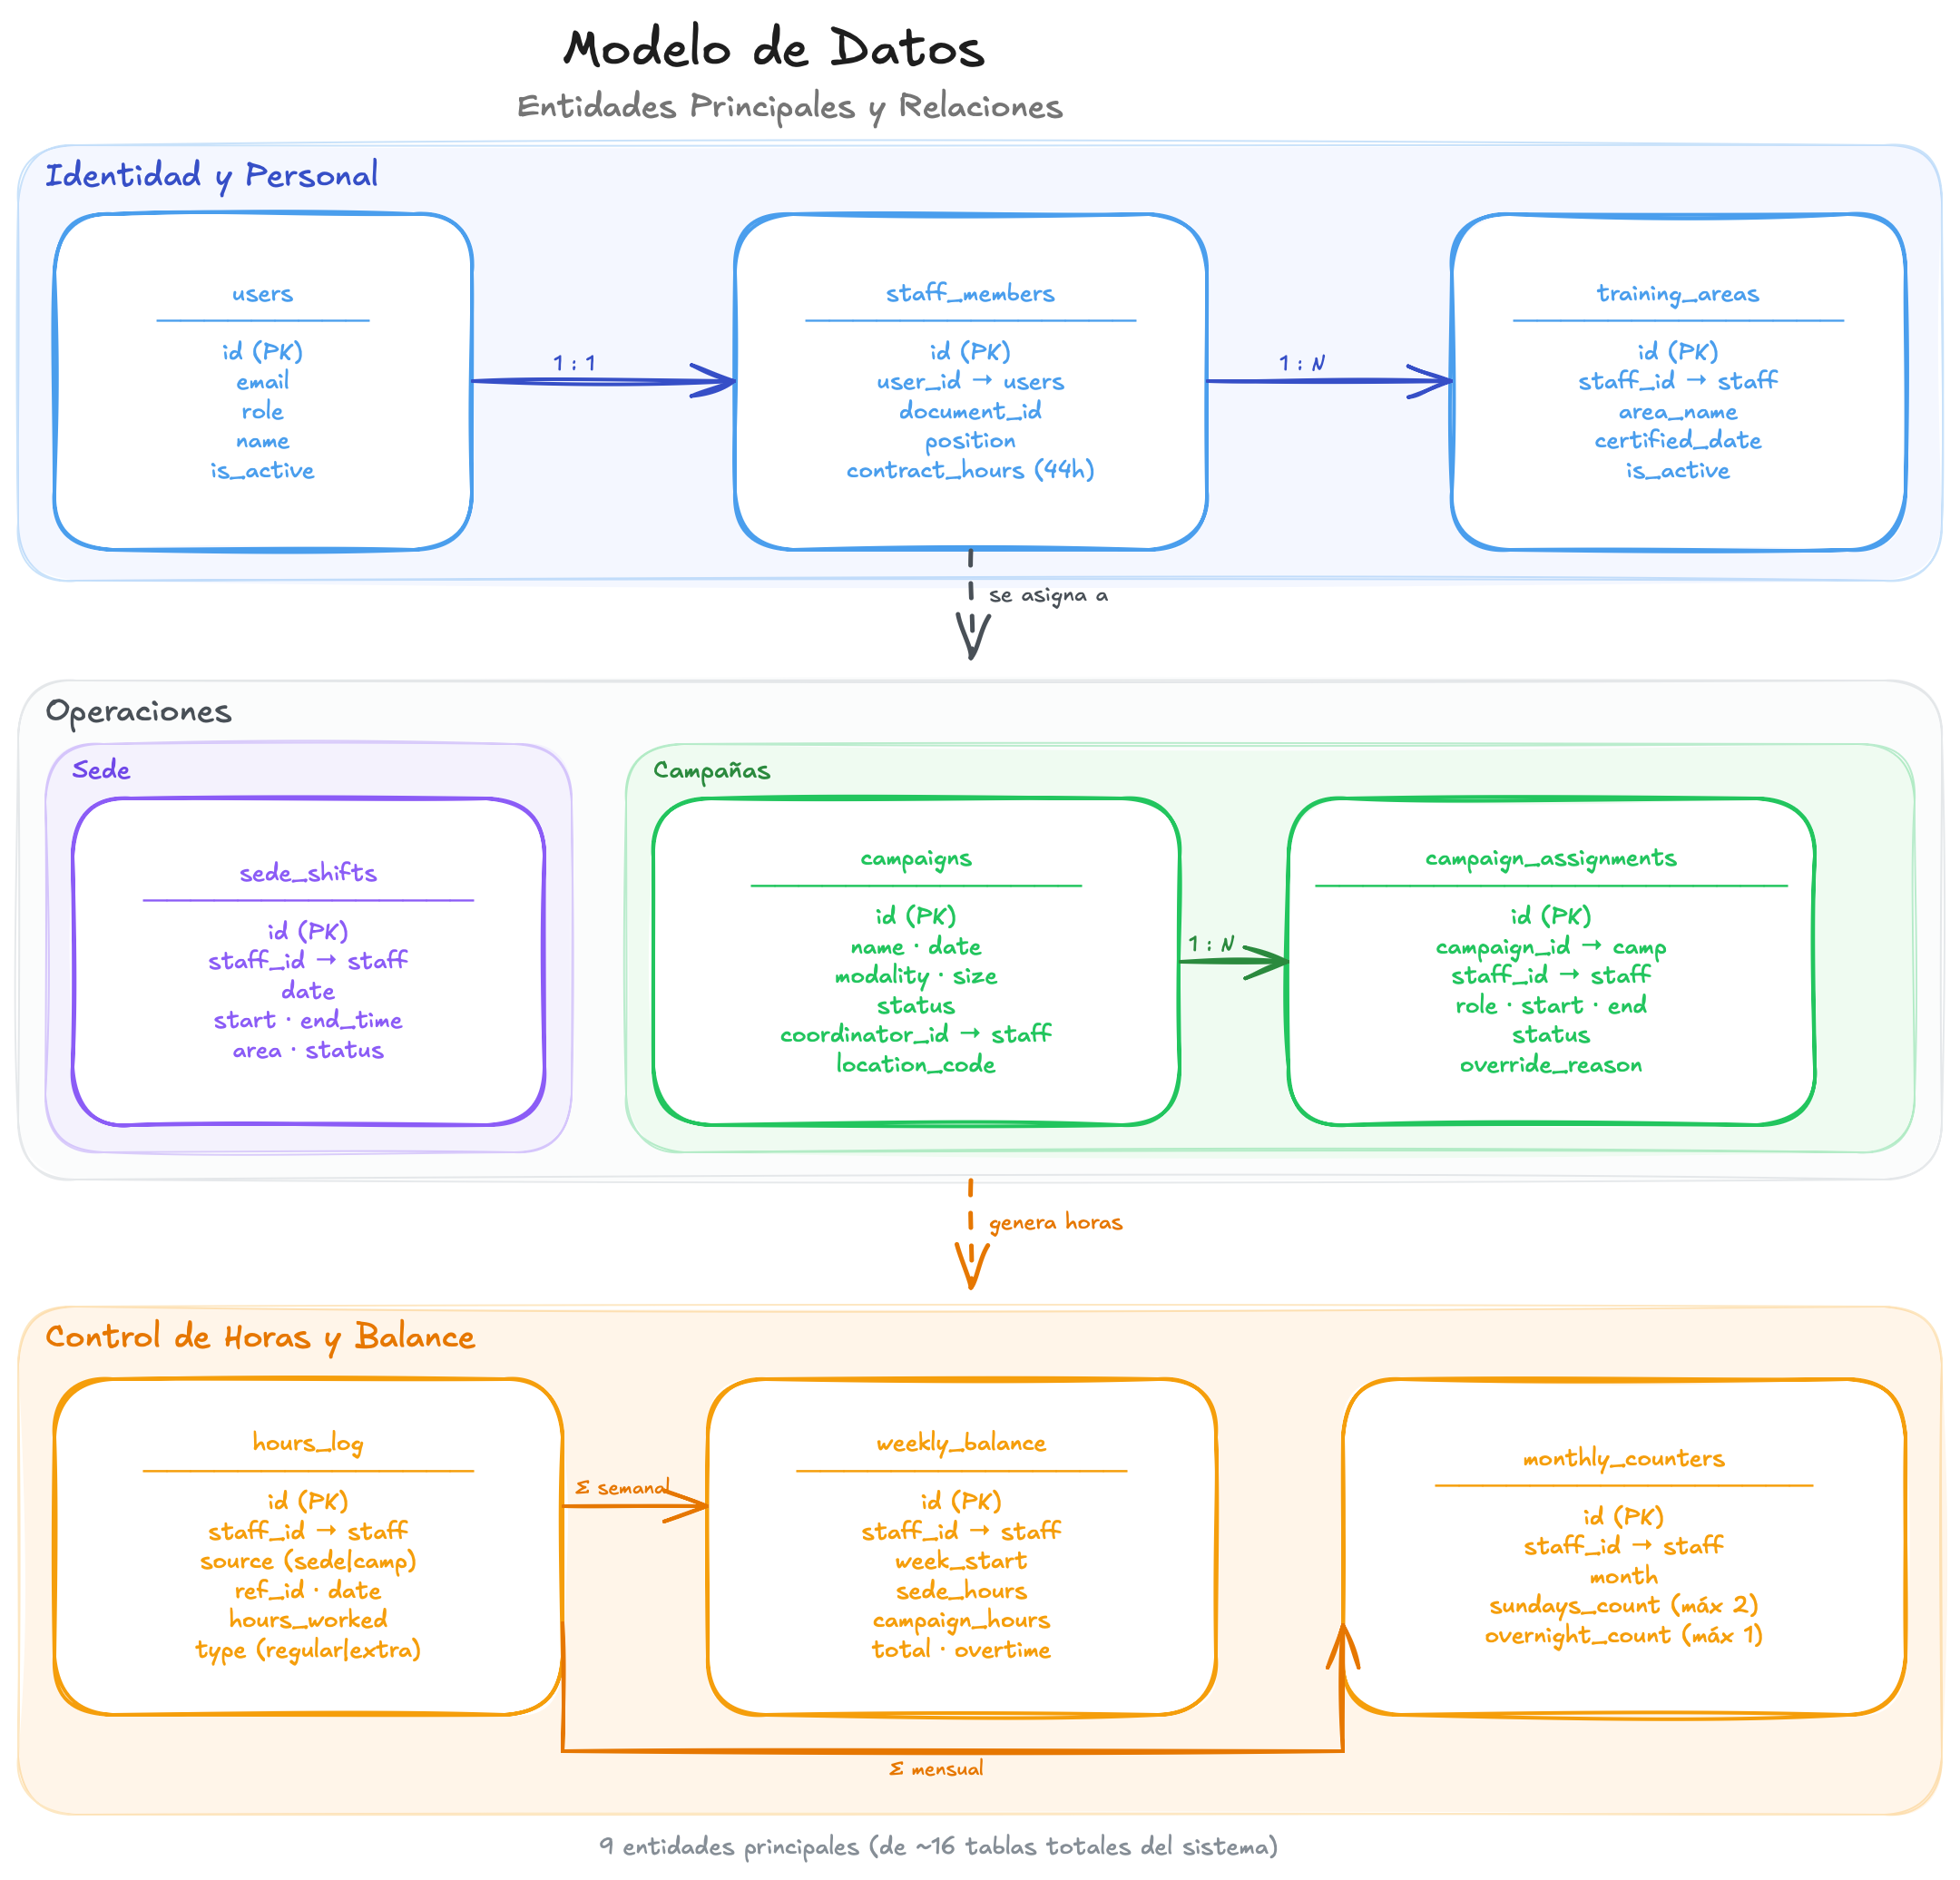
\includegraphics[width=\textwidth]{Untitled-2026-02-11-1419-2.png}
\caption{Modelo de datos: 9 entidades principales en 3 dominios (Identidad, Operaciones, Control de Horas)}
\label{fig:modelo-datos}
\end{figure}

\begin{verbatim}
users 1--M staff_members
staff_members M--M training_areas        (via staff_training_areas)
staff_members 1--M staff_availability
staff_members 1--M sede_shifts           (turnos en sede)
staff_members 1--M campaign_assignments
staff_members 1--M hours_log
staff_members 1--M weekly_balance

campaigns 1--M campaign_assignments
campaigns 1--1 campaign_timeline         (linea de tiempo de horas reales)
campaigns M--1 campaign_coordinator      (designacion, es un staff_id en campaigns)
campaigns M--1 companies                 (empresa solicitante)
campaigns M--1 locations

companies 1--M contacts                  (directorio de contactos)
\end{verbatim}

\subsection{Tablas Principales}

\begin{longtable}{|p{4.2cm}|p{10.3cm}|}
\hline
\textbf{Tabla} & \textbf{Campos Principales} \\
\hline
\endhead
\texttt{users} & id, email, name, role (admin $|$ banco\_sangre $|$ comercial $|$ operativo), is\_active \\
\hline
\texttt{staff\_members} & id, user\_id (FK), document\_number, first\_name, last\_name, phone, profile\_type (bacteriologo $|$ medico $|$ tecnico\_operativo $|$ tecnico\_administrativo), contract\_type, weekly\_contract\_hours (44), max\_overtime\_weekly (12), max\_shift\_hours (12), shift\_type (completo $|$ noche $|$ posturno --- para t\'{e}c. adm.), is\_active \\
\hline
\texttt{training\_areas} & id, code, name, description, is\_active \\
\hline
\texttt{staff\_training\_areas} & id, staff\_id (FK), training\_area\_id (FK), is\_active \\
\hline
\texttt{companies} & id, name, nit, city, municipality, address, contact\_name, contact\_phone, contact\_email, notes, is\_active \\
\hline
\texttt{contacts} & id, company\_id (FK), name, phone, email, position, notes \\
\hline
\texttt{locations} & id, name, address, city, municipality, hexabank\_code, company\_id (FK), notes \\
\hline
\texttt{sede\_shifts} & id, staff\_id (FK), date, shift\_type (completo $|$ noche $|$ posturno), start\_time, end\_time, total\_hours, notes, created\_by\_id (FK) \\
\hline
\texttt{campaigns} & id, code (auto o CRM), company\_id (FK), location\_id (FK), campaign\_size (S $|$ S+ $|$ M $|$ L), modality (corporativa $|$ carpa $|$ unidad\_movil $|$ municipal $|$ combinada), date, start\_time, estimated\_end\_time, requires\_overnight, hexabank\_location\_code, \textbf{coordinator\_id (FK staff\_members)}, status (tentativa $|$ confirmada $|$ cancelada), cancellation\_reason, observations, confirmed\_by\_id (FK), created\_by\_id (FK) \\
\hline
\texttt{campaign\_timeline} & id, campaign\_id (FK), departure\_from\_sede, arrival\_at\_point, campaign\_start, lunch\_start, lunch\_end, campaign\_end, pickup\_time, arrival\_at\_sede, departure\_from\_sede\_end, observations, logged\_by\_id (FK) \\
\hline
\texttt{campaign\_assignments} & id, campaign\_id (FK), staff\_id (FK), role\_in\_campaign, status (asignado $|$ confirmado $|$ completado $|$ no\_asistio), actual\_hours, overtime\_hours, has\_overnight, assigned\_by\_id (FK) \\
\hline
\texttt{hours\_log} & id, staff\_id (FK), date, entry\_type (jornada\_regular $|$ campana $|$ capacitacion $|$ turno\_noche $|$ otro), start\_time, end\_time, total\_hours, regular\_hours, overtime\_hours, surcharge\_type, campaign\_assignment\_id (FK), logged\_by\_id (FK) \\
\hline
\texttt{weekly\_balance} & id, staff\_id (FK), week\_start, week\_end, contracted\_hours (44), worked\_hours, overtime\_hours, balance (positivo: extras $|$ negativo: empleado debe horas), carried\_from\_previous, notes \\
\hline
\texttt{monthly\_counters} & id, staff\_id (FK), month, year, sundays\_worked, overnights\_count \\
\hline
\texttt{staff\_availability} & id, staff\_id (FK), date, start\_time, end\_time, type (disponible $|$ no\_disponible $|$ vacaciones $|$ incapacidad $|$ permiso $|$ jornada\_regular) \\
\hline
\texttt{system\_config} & id, key, value (JSON), description \\
\hline
\texttt{colombian\_holidays} & id, date, name, year \\
\hline
\texttt{audit\_log} & id, user\_id (FK), action, entity\_type, entity\_id, old\_data, new\_data, created\_at \\
\hline
\caption{Esquema de tablas del sistema}
\end{longtable}

\textbf{Nota sobre escalabilidad:} Los campos \texttt{profile\_type}, \texttt{campaign\_size}, \texttt{modality} y las \'{a}reas de entrenamiento se manejan como \textbf{cat\'{a}logos configurables}, permitiendo definir nuevos perfiles, tamaños y modalidades al extender el sistema a otras \'{a}reas sin modificar el c\'{o}digo.

% ══════════════════════════════════════════════════════════════
\section{Estructura de Rutas (Navegaci\'{o}n)}
% ══════════════════════════════════════════════════════════════

\begin{longtable}{|p{5cm}|p{3.5cm}|p{5.5cm}|}
\hline
\textbf{Ruta} & \textbf{Acceso} & \textbf{Descripci\'{o}n} \\
\hline
\endhead
\texttt{/login} & P\'{u}blica & Inicio de sesi\'{o}n \\
\hline
\texttt{/} & Todos & Dashboard principal (adaptado al rol) \\
\hline
\texttt{/campanas} & Admin, BS, Com. & Lista de campañas \\
\hline
\texttt{/campanas/nueva} & Admin, BS & Crear nueva campaña \\
\hline
\texttt{/campanas/[id]} & Admin, BS, Com. & Detalle + asignaci\'{o}n de personal \\
\hline
\texttt{/campanas/importar} & Admin, BS, Com. & Cargar Excel desde CRM \\
\hline
\texttt{/personal} & Admin, BS & Directorio de personal \\
\hline
\texttt{/personal/nuevo} & Admin, BS & Crear empleado \\
\hline
\texttt{/personal/[id]} & Admin, BS, Propio & Detalle de empleado \\
\hline
\texttt{/sede} & Admin, BS & Programaci\'{o}n de turnos en sede \\
\hline
\texttt{/sede/semanal} & Admin, BS & Vista semanal de turnos en sede \\
\hline
\texttt{/programacion} & Admin, BS & Calendario integrado (sede + campañas) \\
\hline
\texttt{/programacion/semanal} & Admin, BS & Tablero semanal de asignaciones \\
\hline
\texttt{/disponibilidad} & Admin, BS, Com. & Dashboard de disponibilidad \\
\hline
\texttt{/reportes/horas} & Admin, BS & Reporte de horas y balance \\
\hline
\texttt{/reportes/campanas} & Admin, BS, Com. & Reporte de campañas \\
\hline
\texttt{/reportes/mensuales} & Admin, BS & Domingos y pernoctas por persona \\
\hline
\texttt{/directorio} & Admin, Com. & Directorio de empresas y contactos \\
\hline
\texttt{/configuracion} & Admin & Configuraci\'{o}n general \\
\hline
\texttt{/configuracion/roles} & Admin & Gesti\'{o}n de usuarios y roles \\
\hline
\texttt{/configuracion/parametros} & Admin & Par\'{a}metros del sistema \\
\hline
\caption{Estructura de rutas del sistema (BS = Banco de Sangre)}
\end{longtable}

% ╔════════════════════════════════════════════════════════════╗
% ║         PARTE IV — IMPLEMENTACI\'{O}N Y CALIDAD              ║
% ╚════════════════════════════════════════════════════════════╝

% ══════════════════════════════════════════════════════════════
\section{Consideraciones de Seguridad}
% ══════════════════════════════════════════════════════════════

\begin{enumerate}[leftmargin=2em]
    \item \textbf{Autenticaci\'{o}n:} Contraseñas hasheadas con bcrypt, tokens de sesi\'{o}n, rate limiting en login.
    \item \textbf{Autorizaci\'{o}n:} Protecci\'{o}n en tres capas: middleware (rutas), componente (UI), server action (datos).
    \item \textbf{Validaci\'{o}n:} Esquemas Zod validados en cliente (formulario) y servidor (acci\'{o}n).
    \item \textbf{Inyecci\'{o}n SQL:} Drizzle ORM usa queries parametrizadas, no SQL crudo.
    \item \textbf{CSRF:} Better Auth gestiona tokens CSRF autom\'{a}ticamente.
    \item \textbf{Auditor\'{i}a:} Todas las mutaciones quedan registradas con usuario, timestamp y datos previos/nuevos.
    \item \textbf{Secretos:} Variables de entorno en \texttt{.env}, nunca en repositorio.
    \item \textbf{Sesiones:} Cookies HTTP-only, flag secure en producci\'{o}n.
    \item \textbf{Datos sensibles:} Los datos de c\'{e}dula y personal solo son visibles para los roles autorizados.
\end{enumerate}

% ══════════════════════════════════════════════════════════════
\section{Plan de Implementaci\'{o}n por Fases}
% ══════════════════════════════════════════════════════════════

\subsection{Fase 1 --- MVP (Semanas 1--4)}

\textbf{Objetivo:} Sistema funcional con gesti\'{o}n de personal, turnos en sede, campañas (3 estados, 3 tamaños, 5 modalidades) y asignaci\'{o}n b\'{a}sica.

\begin{table}[h!]
\centering
\begin{tabularx}{\textwidth}{|c|X|}
\hline
\textbf{Semana} & \textbf{Entregable} \\
\hline
1 & Setup proyecto: Next.js 15, Tailwind, shadcn/ui, Drizzle, PostgreSQL (Docker), Better Auth. Login funcional. Layout dashboard (sidebar + topbar). Seed usuario admin. \\
\hline
2 & M\'{o}dulo Personal: CRUD completo de empleados (crear, editar, eliminar). 4 perfiles. Directorio con DataTable. Asignaci\'{o}n de \'{a}reas de trabajo por administrador. Importaci\'{o}n inicial desde Excel de Banco de Sangre. \\
\hline
3 & M\'{o}dulo Sede: Programaci\'{o}n semanal de turnos en sede (completo, noche, posturno). M\'{o}dulo Campañas: CRUD con 3 estados, 3 tamaños (S/M/L), 5 modalidades. Cat\'{a}logo de empresas. Vista calendario integrado (sede + campañas). Campo Hexabank y observaciones. \\
\hline
4 & Asignaci\'{o}n b\'{a}sica: Asignar personal seg\'{u}n tamaño con designaci\'{o}n de coordinador por campaña. Importaci\'{o}n de Excel desde CRM. Vista de asignaciones. Dashboard con conteos generales. Navegaci\'{o}n por roles (4 roles + coordinador por campaña). \\
\hline
\end{tabularx}
\end{table}

\subsection{Fase 2 --- Motor de Reglas (Semanas 5--8)}

\textbf{Objetivo:} Validaci\'{o}n autom\'{a}tica de reglas laborales (semanales + mensuales), disponibilidad y balance de horas.

\begin{table}[h!]
\centering
\begin{tabularx}{\textwidth}{|c|X|}
\hline
\textbf{Semana} & \textbf{Entregable} \\
\hline
5 & Control de horas: Registro de hora inicio + hora real fin (coordinador). Calculadora de overtime. Balance semanal (cumpli\'{o}/debe/le deben). Contadores mensuales (domingos, pernoctas). Seed festivos 2026. \\
\hline
6 & Asignaci\'{o}n inteligente: Detector de conflictos (9 validaciones). Restricci\'{o}n de municipio. L\'{i}mites mensuales. Proyecci\'{o}n de impacto. Sem\'{a}foro de horas. \\
\hline
7 & Disponibilidad: Matriz visual personal $\times$ fechas. Calendario de capacidad. Tablero semanal. Turnos rotativos de t\'{e}cnicos administrativos. \\
\hline
8 & Flujo comercial completo: Carga semanal Excel $\rightarrow$ creaci\'{o}n de campañas. Vista de personal asignado para Comercial (nombre, CC, cargo). Directorio de empresas/contactos. \\
\hline
\end{tabularx}
\end{table}

\subsection{Fase 3 --- Reportes e Integraci\'{o}n (Semanas 9--12)}

\textbf{Objetivo:} Visibilidad de datos, integraci\'{o}n Excel bidireccional, auditor\'{i}a y notificaciones.

\begin{table}[h!]
\centering
\begin{tabularx}{\textwidth}{|c|X|}
\hline
\textbf{Semana} & \textbf{Entregable} \\
\hline
9 & Reportes: Horas con balance semanal, campañas, horas extras, pernoctas y domingos mensuales. \\
\hline
10 & Excel bidireccional: Exportaci\'{o}n de reportes. Importaci\'{o}n de personal, \'{a}reas, campañas CRM. Plantillas. Validaci\'{o}n. \\
\hline
11 & Auditor\'{i}a y operaciones: Log de auditor\'{i}a. Cancelaci\'{o}n con impacto. Datos de Hexabank (c\'{o}digo de lugar). Migraci\'{o}n de directorio de contactos. \\
\hline
12 & UX: Notificaciones in-app. Alertas de horas extras, domingos y pernoctas. Diseño responsive. Estados de carga y vac\'{i}os. \\
\hline
\end{tabularx}
\end{table}

\subsection{Fase 4 --- Funcionalidades Avanzadas (Semanas 13--16)}

\textbf{Objetivo:} Anal\'{i}tica, optimizaci\'{o}n e integraci\'{o}n avanzada con Hexabank.

\begin{table}[h!]
\centering
\begin{tabularx}{\textwidth}{|c|X|}
\hline
\textbf{Semana} & \textbf{Entregable} \\
\hline
13 & Dashboard anal\'{i}tico: M\'{e}tricas de campañas, utilizaci\'{o}n de personal, tendencias de overtime, domingos/pernoctas. \\
\hline
14 & Asignaci\'{o}n sugerida: Auto-sugerencia por disponibilidad, overtime, equidad y balance. Simulador. \\
\hline
15 & Avanzado: Integraci\'{o}n Hexabank (donantes, c\'{o}digos). Templates recurrentes. Exportaci\'{o}n iCal. Vistas m\'{o}vil. \\
\hline
16 & Cierre: Testing E2E. Documentaci\'{o}n de usuario. Optimizaci\'{o}n. Revisi\'{o}n de seguridad. Deploy a producci\'{o}n. \\
\hline
\end{tabularx}
\end{table}

% ══════════════════════════════════════════════════════════════
\section{Verificaci\'{o}n y Pruebas}
% ══════════════════════════════════════════════════════════════

Para validar que el sistema funciona correctamente de extremo a extremo:

\begin{enumerate}[leftmargin=2em]
    \item \textbf{Auth:} Login con cada uno de los 4 roles; verificar que solo ven las rutas permitidas.
    \item \textbf{Personal:} Crear bacteri\'{o}logo, m\'{e}dico, t\'{e}cnico operativo y t\'{e}cnico administrativo con \'{a}reas habilitadas diferentes.
    \item \textbf{Sede:} Programar turnos semanales en sede; verificar que las horas se suman al c\'{o}mputo semanal.
    \item \textbf{Sede + Campaña:} Asignar a campaña a una persona con turno de sede ese d\'{i}a; verificar que el turno de sede se ajusta.
    \item \textbf{Campaña:} Crear campaña S, M y L con diferentes modalidades; verificar composici\'{o}n de equipo.
    \item \textbf{Importaci\'{o}n CRM:} Cargar Excel de prueba con 5 campañas; verificar que se crean como tentativas.
    \item \textbf{Asignaci\'{o}n:} Asignar personal; verificar que bloquea por \'{a}rea no habilitada y advierte por overtime.
    \item \textbf{Coordinador:} Designar coordinador por campaña; verificar que solo puede registrar horas de esa campaña espec\'{i}fica y no de otras.
    \item \textbf{Municipio:} Asignar a campaña municipal y verificar restricci\'{o}n del d\'{i}a anterior (max 5pm).
    \item \textbf{Domingos:} Asignar a 3 campañas dominicales; verificar que la tercera genera advertencia.
    \item \textbf{Pernoctas:} Asignar a 2 campañas con pernocta; verificar que la segunda genera advertencia.
    \item \textbf{Balance:} Simular semana con 24h sede + 16h campaña = 40h; verificar ``le deben 4h'' y que se arrastra.
    \item \textbf{Hora real:} Coordinador registra hora real de fin; verificar que actualiza horas y balance de todo el equipo.
    \item \textbf{Comercial:} Verificar que puede ver nombre, c\'{e}dula y cargo del personal asignado.
    \item \textbf{Reportes:} Generar reporte semanal con columnas sede + campaña + balance; exportar a Excel.
    \item \textbf{Cancelaci\'{o}n:} Cancelar campaña con asignaciones; verificar liberaci\'{o}n de horas y ajuste de balance.
    \item \textbf{Hexabank:} Verificar que el c\'{o}digo de lugar se registra y se muestra correctamente.
\end{enumerate}

\vfill

\begin{center}
    {\color{azuloscuro}\rule{0.5\textwidth}{1pt}}\\[0.5cm]
    {\small\color{grisoscuro} Documento generado por el \'{A}rea de Transformaci\'{o}n Digital\\
    Cruz Roja Colombiana Seccional Antioquia --- Febrero 2026\\
    Versi\'{o}n 3.0}
\end{center}

\end{document}
